\section{Experiments} \label{sec:experiments}

In what follows we empirically probe properties of the MIM model,
with the VAE as a baseline.  We consider both low-dimensional synthetic 
datasets and well-known images datasets, including MNIST \cite{LeCun1998}, 
Fashion MNIST \cite{DBLP:journals/corr/abs-1708-07747} and Omniglot \cite{Lake2015}. 
The code used to generate the results reported below is available 
from \href{https://github.com/seraphlabs-ca/MIM}{https://github.com/seraphlabs-ca/MIM}.
In all experiments (unless otherwise specified) we use Adam optimizer \cite{2014arXiv1412.6980K} with $lr = 1e-3$, and
mini-batch of size 128. We stopped training for all experiments when validation loss
has not improved for 10 epochs.

%%%%%%%%%%%%%%%%%%%%%%%%%%%%%%%%%%%%%%%%%%%%%%%%%%%%%%%%
% \subsection{Posterior Collapse in MIM and VAE} 
\subsection{2D Mixture Model Data} 
\label{sec:posterior-collapse-mim-vae}


We begin with a synthetic dataset of 2D observations $\x \in \mathbb{R}^2$
and a 2D latent space, $\z \in \mathbb{R}^2$. In two dimensions we can easily 
visualize the model and measure quantitative properties of interest (\eg, mutual information).
Data are drawn from a Gaussian mixture model with five isotropic components
with standard deviation 0.25; the black contours in Fig.\ \ref{fig:posterior-collapse-qualitative} (top) depict level sets of constant density $\pjoint(\x)$. 
The latent anchor, $\pjoint(\z)$, is an isotropic standard normal distribution.
The encoder and decoder conditional distributions are Gaussian, the means
and variances of which are regressed from the input using two fully 
connected layers and swish activation \cite{Ramachandran2017}).
Finally, the parameterized data prior, $\Menc(\x)$, is defined to be the 
marginal of the decoding distribution \eqref{eqn:q-marginal}, so
the only model parameters are those of the encoder and decoder.
As such we can learn models with MIM and VAE objective that share
the same architectures and parameterizations.

Figure \ref{fig:posterior-collapse-qualitative} depicts four models 
for the VAE (top two rows) and MIM (bottom rows), with increasing numbers 
of hidden units (moving left to right) to control model expressiveness.
The first and third rows (for VAE and MIM respectively) depict observation 
space where black contours are levels sets of constant density 
$\pjoint (\x)$, and red points are reconstructed samples, 
i.e., one point drawn from the decoder $\Mdec(\x | \z' )$ where $\z'$ is 
drawn from the encoder $ \Menc(\z' | \x') $, given observation $\x'$ 
from $\pjoint(\x)$ in the test set.
With each case we report the mean squared reconstruction error, which are 
lower for MIM than VAE. 


\begin{figure}[t]
    \centering
    \setlength{\tabcolsep}{0pt}
    \begin{tabular}{*6{>{\centering\arraybackslash}m{0.167\textwidth}}}
      {\scriptsize VAE} & {\scriptsize MIM} & {\scriptsize VAE} & {\scriptsize MIM} & {\scriptsize VAE} & {\scriptsize MIM} \\
      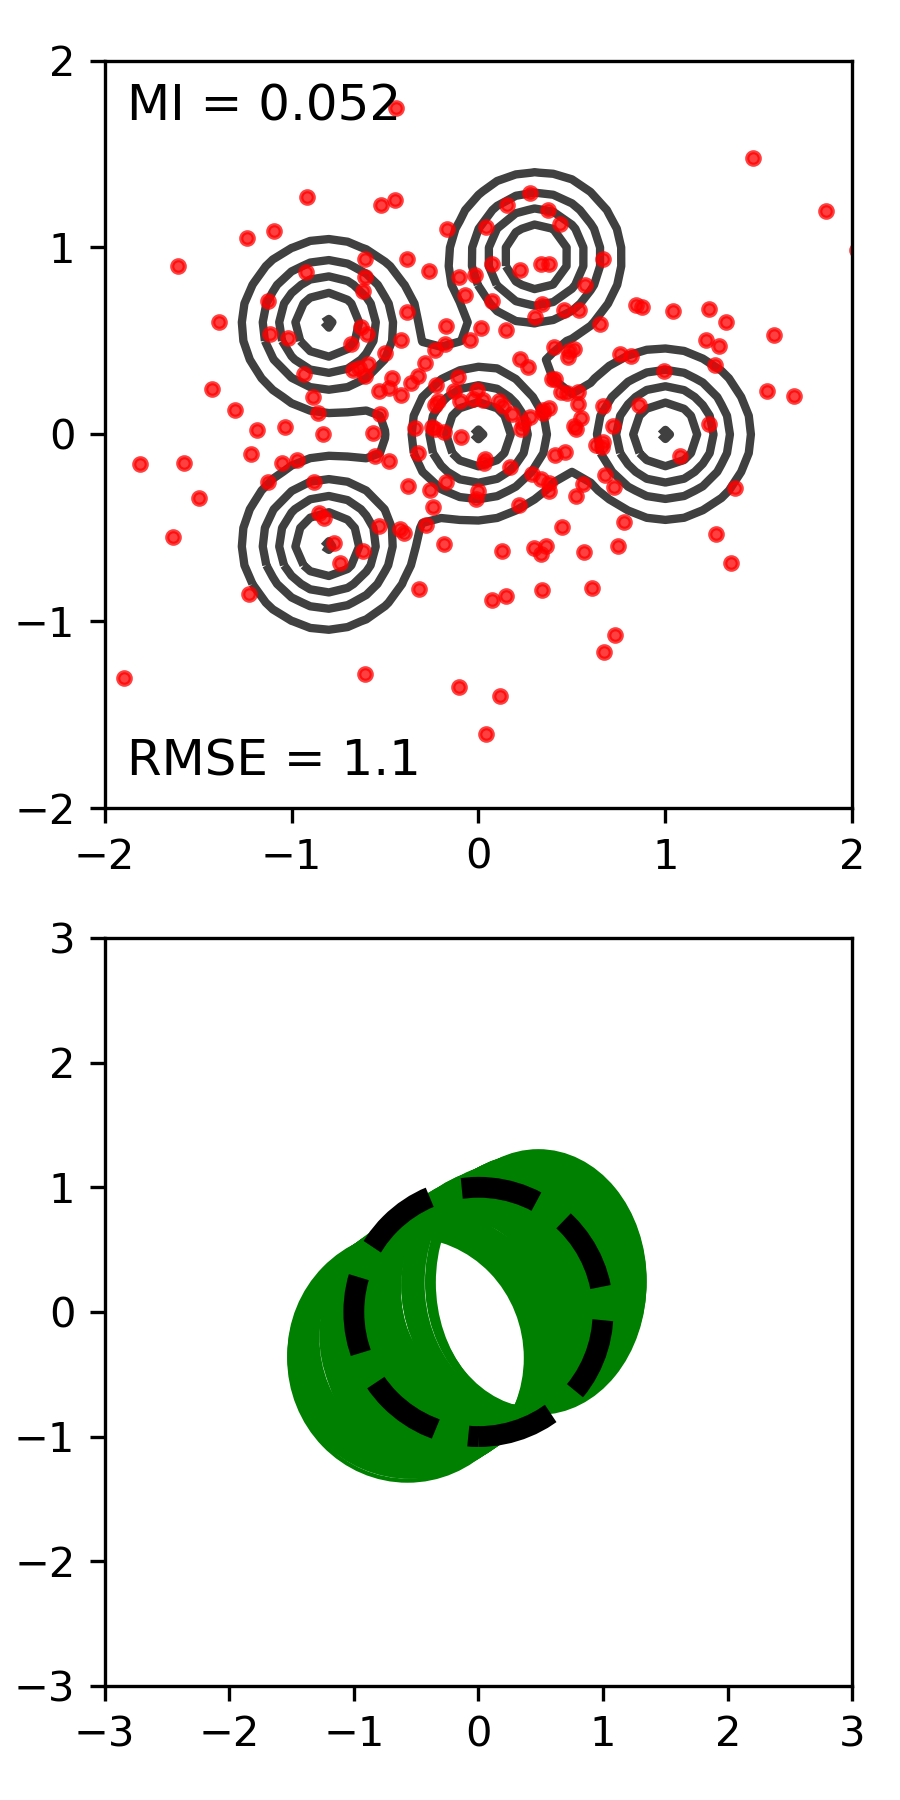
\includegraphics[width=0.165\columnwidth]{images/vae-as-mim-toy-2d/toy4/plots/vae_logvar10_mid-dim5_layers2_q-x0marginal_q-zx0_p-z0anchor_p-xz0/reconstruction_best.png}
    & 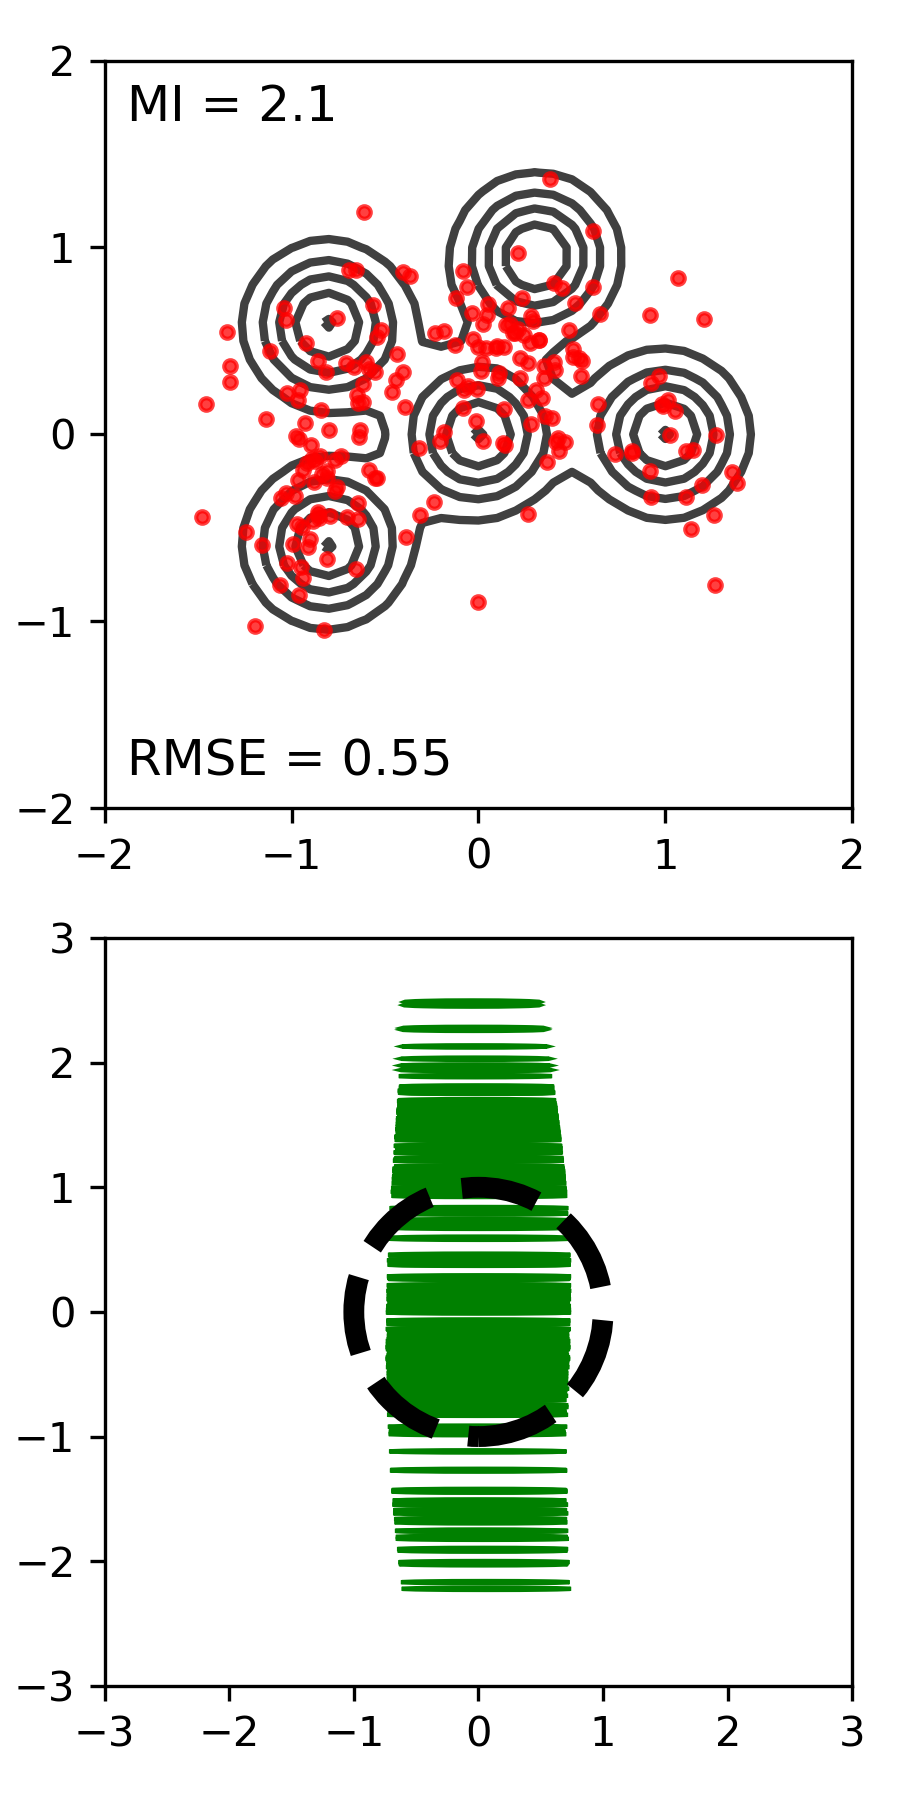
\includegraphics[width=0.165\columnwidth]{images/vae-as-mim-toy-2d/toy4/plots/mim-samp_logvar10_mid-dim5_layers2_q-x0marginal_q-zx0_p-z0anchor_p-xz0/reconstruction_best.png}
    & 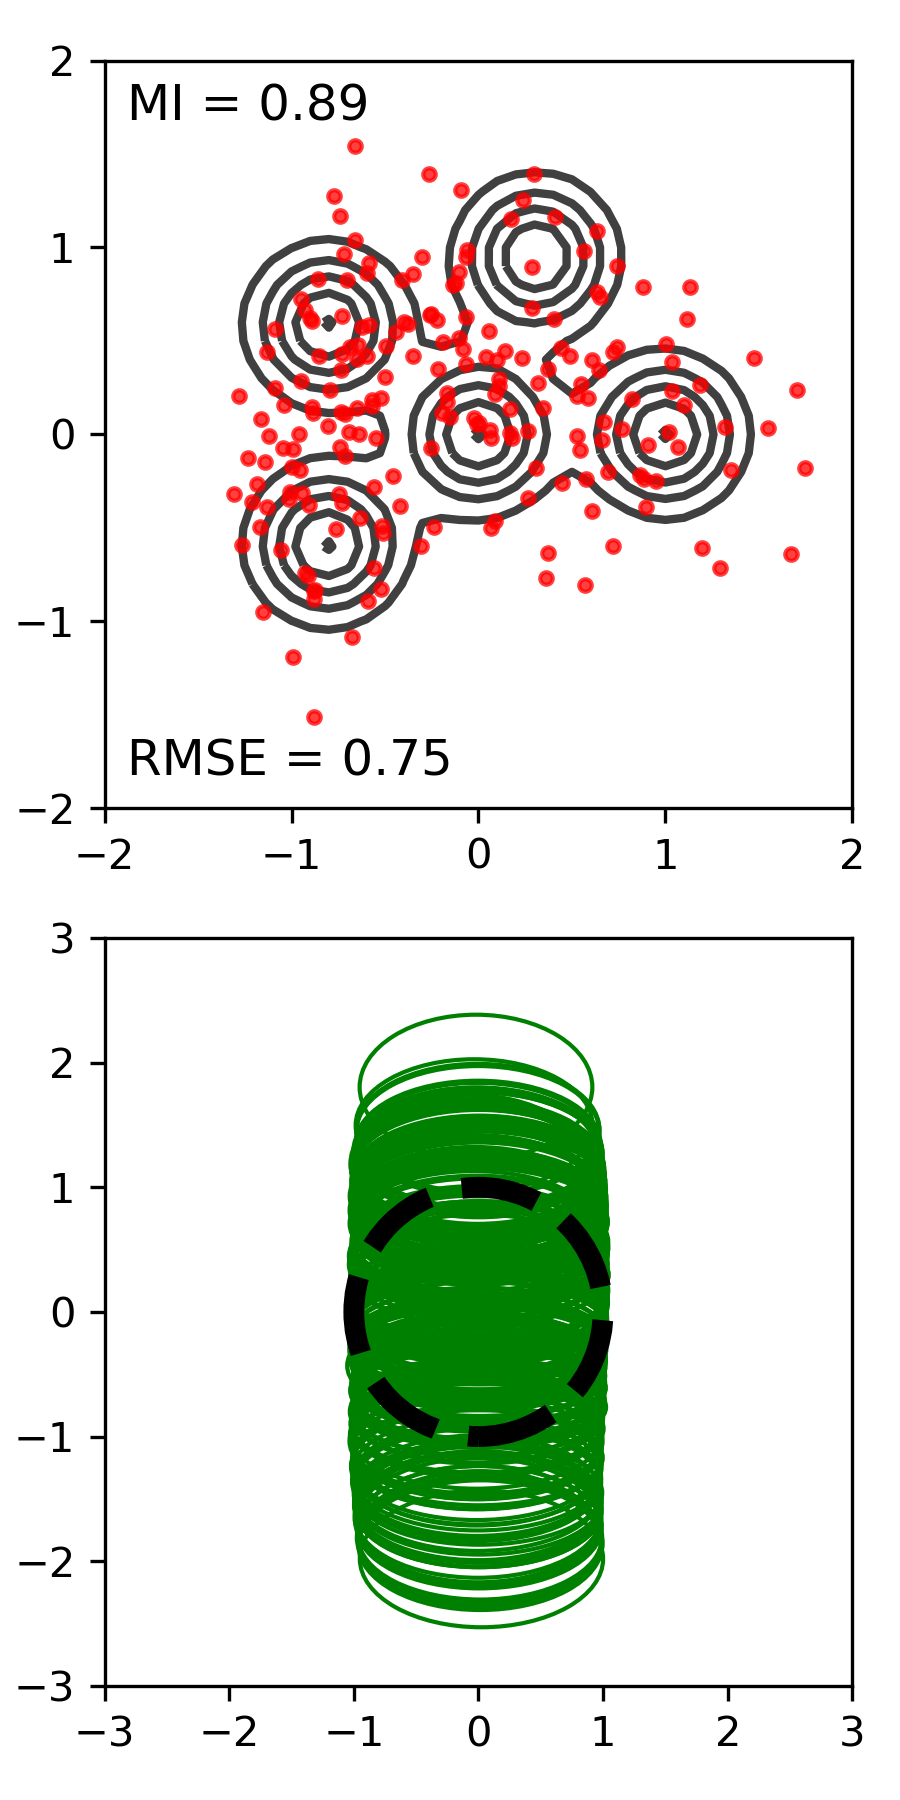
\includegraphics[width=0.165\columnwidth]{images/vae-as-mim-toy-2d/toy4/plots/vae_logvar10_mid-dim20_layers2_q-x0marginal_q-zx0_p-z0anchor_p-xz0/reconstruction_best.png}
    & 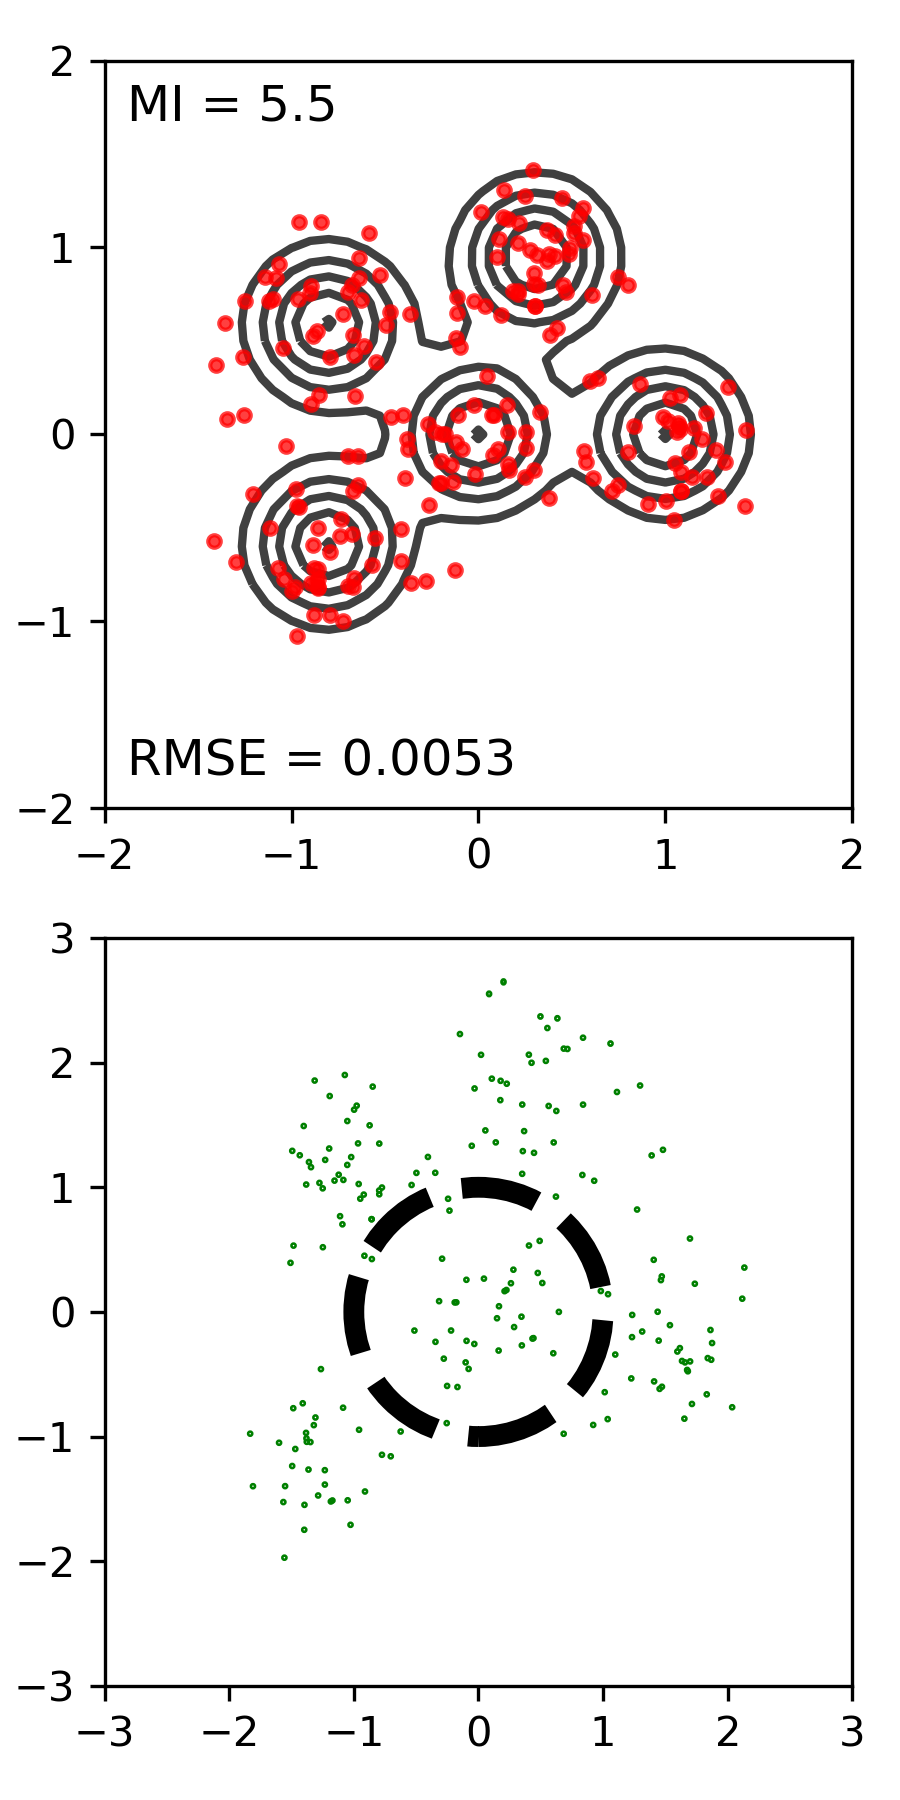
\includegraphics[width=0.165\columnwidth]{images/vae-as-mim-toy-2d/toy4/plots/mim-samp_logvar10_mid-dim20_layers2_q-x0marginal_q-zx0_p-z0anchor_p-xz0/reconstruction_best.png}
    & 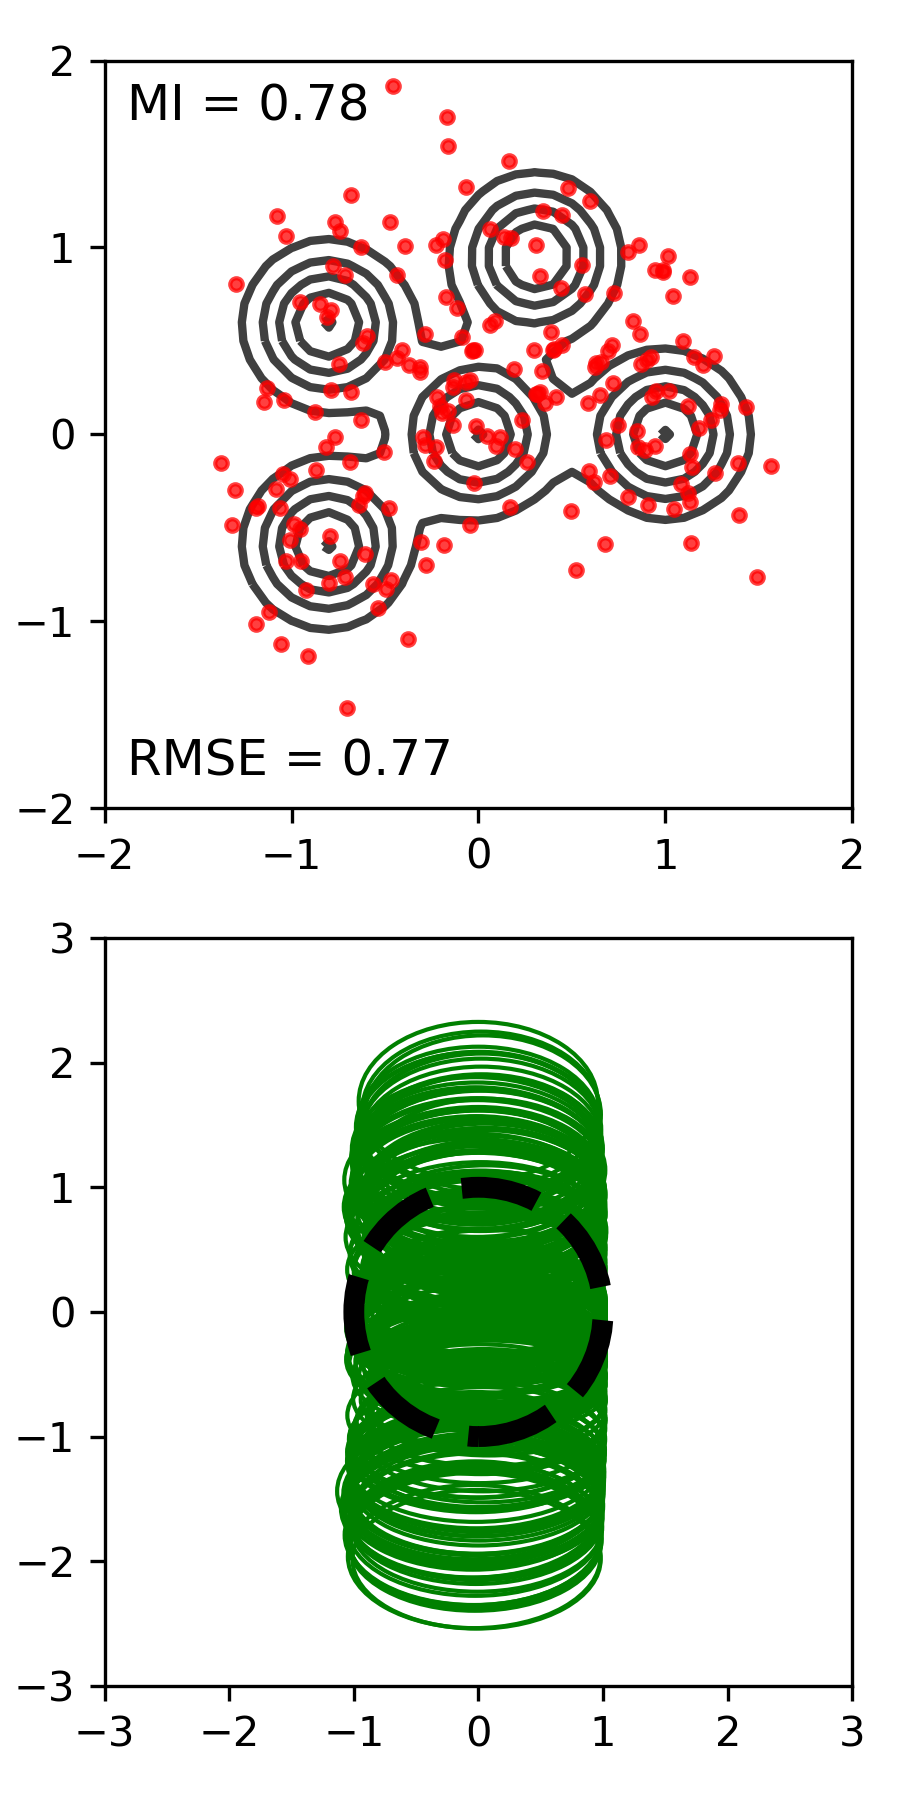
\includegraphics[width=0.165\columnwidth]{images/vae-as-mim-toy-2d/toy4/plots/vae_logvar10_mid-dim500_layers2_q-x0marginal_q-zx0_p-z0anchor_p-xz0/reconstruction_best.png}
    & 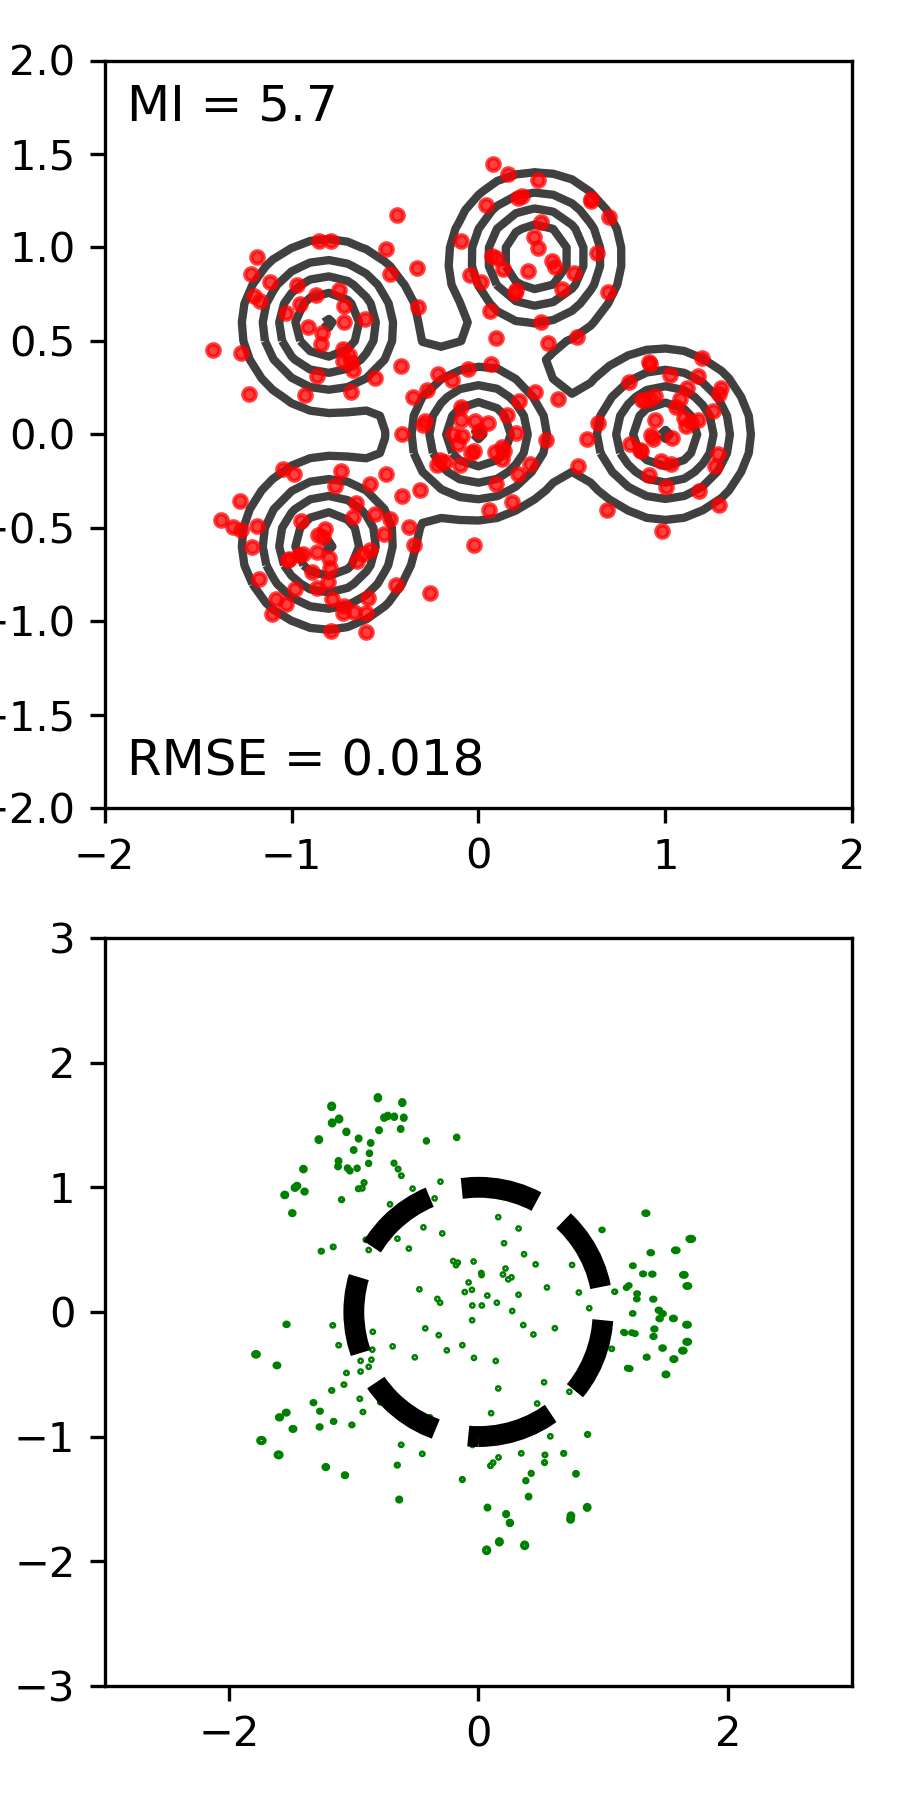
\includegraphics[width=0.165\columnwidth]{images/vae-as-mim-toy-2d/toy4/plots/mim-samp_logvar10_mid-dim500_layers2_q-x0marginal_q-zx0_p-z0anchor_p-xz0/reconstruction_best.png}
    \\
    \multicolumn{2}{c}{(a) $h \in \mathbb{R}^{5}$ } & \multicolumn{2}{c}{(b) $h \in \mathbb{R}^{20}$ } & \multicolumn{2}{c}{(c) $h \in \mathbb{R}^{500}$ } \\
    \end{tabular}
    \caption{
    VAE and MIM models with 2D inputs, a 2D latent space, and 5, 20 and 500 hidden units. 
    Top row: Black contours depict level sets of $\pjoint(\x)$, red points are 
    reconstructed test points.
    Bottom row: Green contours are one standard deviation ellipses of 
    $\Menc(\z|\x)$ for test points. Dashed black circles depict one standard 
    deviation of $\pjoint (\z)$.
    (a) For weak architectures MIM and VAE exhibit high posterior variance.
    (b,c) For more expressive architectures the VAE predictive variance remains high,
    an indication of posterior collapse.
    MIM generally produces lower predictive variance and lower reconstruction 
    errors, consistent with high mutual information (see inset quantities).
    \david{can y axis be same as x-axes on top plots ... no decimal?}
    }\label{fig:posterior-collapse-qualitative}
\end{figure}

% \begin{figure}[t]
%     \centering
%     \setlength{\tabcolsep}{0pt}
%     \begin{tabular}{m{0.12\textwidth} *4{>{\centering\arraybackslash}m{0.22\textwidth}}}
%     {(i) VAE}
%     & \includegraphics[width=0.22\columnwidth]{images/vae-as-mim-toy-2d/toy4/z2/vae_logvar10_mid-dim5/reconstruction_200.png}
%     & \includegraphics[width=0.22\columnwidth]{images/vae-as-mim-toy-2d/toy4/z2/vae_logvar10_mid-dim20/reconstruction_200.png}
%     & \includegraphics[width=0.22\columnwidth]{images/vae-as-mim-toy-2d/toy4/z2/vae_logvar10_mid-dim100/reconstruction_200.png}
%     & \includegraphics[width=0.22\columnwidth]{images/vae-as-mim-toy-2d/toy4/z2/vae_logvar10_mid-dim500/reconstruction_200.png}
%     \\
%     {(ii) \MIM}
%     & \includegraphics[width=0.22\columnwidth]{images/vae-as-mim-toy-2d/toy4/z2/mim-samp_logvar10_mid-dim5/reconstruction_200.png}
%     & \includegraphics[width=0.22\columnwidth]{images/vae-as-mim-toy-2d/toy4/z2/mim-samp_logvar10_mid-dim20/reconstruction_200.png}
%     & \includegraphics[width=0.22\columnwidth]{images/vae-as-mim-toy-2d/toy4/z2/mim-samp_logvar10_mid-dim100/reconstruction_200.png}
%     & \includegraphics[width=0.22\columnwidth]{images/vae-as-mim-toy-2d/toy4/z2/mim-samp_logvar10_mid-dim500/reconstruction_200.png}
%     \\
%     & (a) $h \in \mathbb{R}^{5}$  & (b) $h \in \mathbb{R}^{20}$ & (c) $h \in \mathbb{R}^{100}$ & (d) $h \in \mathbb{R}^{500}$
%     \end{tabular}
%     \caption{
%     (i) VAE vs (ii) MIM with 2D inputs and 2D latent spaces, and different 
%     numbers of hidden units (columns (a) -- (d)).
%     Rows 1, 3: Black contours depict level sets of $\pjoint(\x)$, red points
%     are reconstructed test points, with average reconstruction error inset.
%     Rows 2, 4: Green contours are one standard deviation ellipses of 
%     $\Menc(\z|\x)$ for test points. Dashed black circles depict one standard 
%     deviation of $\pjoint (\z)$.
%     For weak architectures (a) MIM and VAE have very high posterior variance.
%     For more expressive architectures the predictive variance remains high 
%     for the VAE. With $h=500$ the VAE also finds solutions like that in (b), 
%     a clear sign of posterior collapse. 
%     % We posit that such high posterior variance is due to the mutual 
%     % information term in the objective \eqref{eq:vi-as-ml-objective-text}. 
%     MIM generally produces lower predictive variance and lower reconstruction 
%     errors in (b)-(d), consistent with high mutual information.
%     }\label{fig:posterior-collapse-qualitative}
% \end{figure}

\begin{figure}[ht]
    \centering
    \setlength{\tabcolsep}{0pt}
    \begin{tabular}{*4{>{\centering\arraybackslash}m{0.24\textwidth}}}
      \includegraphics[width=0.2\columnwidth]{{images/vae-as-mim-toy-2d/toy4/stats/fig.MI_ksg}.png}
    & \includegraphics[width=0.2\columnwidth]{{images/vae-as-mim-toy-2d/toy4/stats/fig.H_q_x.symlog}.png}
    & \includegraphics[width=0.2\columnwidth]{{images/vae-as-mim-toy-2d/toy4/stats/fig.x_recon_err.symlog}.png}
        & \includegraphics[width=0.2\columnwidth]{{images/vae-as-mim-toy-2d/toy4/stats/fig.clf_acc_KNN5}.png}
    \\
    (a) MI & (b)  ELBO & (c) Recon.\ Error & (d) Classif.\ (5-NN)
    \end{tabular}
    \caption{Test performance for MIM (blue) and VAE (red) for 2D GMM experiment,
    all as functions of the number of hidden units (on x-axis). From left to right,
    plots show mutual information, log marginal probability of test points,  is MIM, red is VAE, the graphs depict mean and standard deviation of 10 experiments. (c-d) are shown with logarithmic scale.
    \david{change elbo to ave log marginal likelihood.}
    }\label{fig:posterior-collapse-quantitative}
\end{figure}

% \begin{figure}[h!]
%     \centering
%     \begin{minipage}[b]{0.5\columnwidth}
%     \centering
%     \scalebox{0.9}[0.9]{\input{diag/posterior-collapse-mi}}
%     \label{fig:posterior-collapse-quantitative-mi}
%     \end{minipage}%
%     \begin{minipage}[b]{0.5\columnwidth}
%     \centering
%     \scalebox{0.9}[0.9]{\input{diag/posterior-collapse-log_p_x}}
%     \label{fig:posterior-collapse-quantitative-log-p-x}
%     \end{minipage}
%     \caption{
%     Mutual information (left) and data log likelihood (right) for 
%     MIM and VAE, for different numbers of hidden units. Plots show means and
%     min-max intervals over 10 models learned from different random datasets.
%     MIM tends to produce higher mutual information and log likelihoods.
%     \micha{Will be replaced with plots similar to \ref{fig:mim-vs-vae-image-quantitative-bottleneck}}
%     % Bars represent the mean over 10 independently trained models, along with min-max interval.
%     % Surprisingly, a more expressive VAE leads to a slightly lower data marginal, where the added expressiveness is utilized to increase the encoder conditional entropy (second row in Fig. \ref{fig:posterior-collapse-qualitative}). Mutual information values in VAE are mostly unaffected and stays around the level that allows good reconstruction.
%     % \micha{show KL divergence of posterior vs prior (?? see results in report. Do we need it?)}\micha{H(P(x)) = 1.3859}
%     }\label{fig:posterior-collapse-quantitative}
% \end{figure}




Rows 2 and 4 of Fig.\ \ref{fig:posterior-collapse-qualitative}
depict the latent space behavior.  The dashed black circle 
depicts one standard deviation of $\pjoint(\z)$. Each green 
curve depicts a one standard deviation ellipse of the encoder posterior  
$\Menc(\z' | \x')$ for a data point $\x'$ drawn from $\pjoint(\x)$.
One can clearly see that for the weakest architecture, with only 5 
hidden units, both MIM and VAE posteriors have large variances.
When the number of hidden units increases to 20, however, it is 
clear that will the VAE posterior variance remains very large in
one dimension, the MIM encoder produces much tighter posteriors 
densities.  Even though VAE posteriors become somewhat tighter with even
more expressive models, compared to MIM, they continue to exhibit
very high variances, a common sign of posterior collapse. 



To quantify this behavior for each architecture in  
Fig.\ \ref{fig:posterior-collapse-qualitative}, Fig.\ 
\ref{fig:posterior-collapse-quantitative} plots the mutual information, 
the average log marginal of test points under the model $\Menc$,
the reconstruction error of test points, and 5-NN classification
(predicting which of five GMM components the test points were drawn from).
Following  \cite{Hjelm2018}, we estimate mutual information 
using the KSG mutual information estimator \cite{PhysRevE.69.066138,DBLP:journals/corr/GaoOV16},  
based on a K-NN neighborhoods with $k=5$, and measure the quality of the representation with classification axuliary task.

One can see that mutual information and the average log likelihood 
of the test data under the MIM model are higher than for VAE models.
One can also see that mutual information saturates for MIM as the
number of hidden units grow larger than 20.
(We direct the reader to Sec.\ \ref{sec:entropy-as-mi-regularizer}
of the supplementary material for experiments on variants of 
MIM and VAE tease apart the impact of specific terms of the 
respective objectives.)

One can also see from Fig.\ \ref{fig:posterior-collapse-qualitative} that as the models 
becomes sufficiently expressive, in terms of the number of 
hidden units, the MIM encoding variance becomes extremely small,
and the reconstruction error in Fig.\ \ref{fig:posterior-collapse-quantitative} approaches 0.
Effectively, the encoder and decoder learn an (approximately) invertible mapping using 
an unconstrained architecture (demonstrated here for the 2D case), when the 
dimensionality of the latent representation and the observations is the same.

% One can also see from Fig.\ \ref{fig:posterior-collapse-quantitative} that
% as the model becomes sufficiently expressive, in terms of the number of 
% hidden units, the MIM reconstruction error approaches that of a similarly 
% expressive deterministic autoencoder. In effective, the MIM encoder becomes 
% a delta function around a deterministic mapping.
% % $\Menc(\z|\x) \rightarrow \delta \left( \z - f_{\Menc}(\x) \right)$. 

The VAE, by comparison, is prone to posterior collapse, with latent embeddings 
with relatively low mutual information. In regard, we note that several 
papers have described ways to mitigate posterior collapse in VAE learning, e.g., 
by lower bounding, or annealing the KL divergence term in the VAE objective 
(e.g., \citep{DBLP:journals/corr/abs-1711-00464,DBLP:journals/corr/abs-1901-03416}), 
or by limiting the expressiveness of the decoder (e.g., \citep{ChenKSDDSSA16}).
We posit that MIM does not suffer from this problem as a consequence of 
the objective design principles that encourage high mutual information
between observations and the latent representation.


% Posterior collapse in 2D $\x$ and 2D $\z$ toy problem with $\pjoint(\x)$ being a GMM with 5 components, $\pjoint(\z) = \pdec(\z)$ is a Normal distribution, and the encoder and decoder are conditional Gaussians (regressors are 2 FC layers and swish activation \cite{Ramachandran2017}). \textcolor{red}{$\blacksquare$} Odd rows depict $\pjoint(\x)$ data distribution (black iso-contours) and reconstruction samples $\x_{i} \sim \Mdec(\x|\z_{i})$ (red points). \micha{We need to add how to fake q(x).} \textcolor{OliveGreen}{$\blacksquare$} Even rows depict the Normal prior $p(\z)$ (dashed black line), and the corresponding posterior $\z_{i} \sim \Menc(\z|\x)$ (green ellipses), where each ellipse has mean and principal axis which are the mean and standard deviation of the posterior. In this experiment we compare a VAE model trained with VI in row (i) with the same model in row (ii) trained as \MIM (\ie, by approximating $\log \Menc(\x) \approx \log \E{\z \sim p(\z)}{\Mdec(\x|\z)}$). \micha{this also shows that VAE model can be easily trained as MIM. See \ref{algo:vae-as-mim}} Also we define the prior to be the anchor $p(\z) = \pjoint(\z) = \mathcal{N}(\z)$. Row (iii) summarizes the corresponding statistics. Columns (a-d) vary the size of the hidden layer in the regressors, where larger dimensionality translates into a more expressive model.
% \textbf{(i)} Posterior collapse in VAE  with limited expressiveness (a-b), and partial collapse with an over-expressive model (d). In (c) the posterior successfully capture the structure of the observations.
% \textbf{(ii)} \MIM demonstrates higher MI in all cases, in addition to robustness to posterior collapse for over-expressive models. The higher MI is visualize by the structure in the latent space which captures the observations structure, while aligned to approximate the prior $p(\z)$. In (a) the model expressiveness is limited, and the model utilizes only 1 dimension to capture the observations structure.
% \textbf{(iii)} (e-f) It is clear that \MIM training results in higher MI, which is capped for over-expressive models due to the consistency regularizer. This stands in contrast to VAE which is sensitive to under and over expressiveness. (g-h) Compare to VAE, \MIM has higher data log likelihood which grows with model expressiveness, while VAE suffers from posterior collapse which results in lower data likelihood. (j-k) Interestingly enough, both \MIM and VAE can better match the posterior to the prior over $\z$ with more expressive models, where \MIM posterior matches the prior worse when compared with VAE.



%%%%%%%%%%%%%%%%%%%%%%%%%%%%%%%%%%%%%%%%%%%%%%%%%%%%%%%%
\subsection{Bottleneck}
% \subsection{Experiments with Bottleneck on GMM and Subspace Fashion MNIST.}

\begin{figure}[t]
    \centering
    \setlength{\tabcolsep}{0pt}
    \begin{tabular}{*4{>{\centering\arraybackslash}m{0.25\textwidth}}}
      \includegraphics[width=0.25\columnwidth]{{images/vae-as-mim-pca/fashion-mnist/fig.MI_ksg}.png}
    & \includegraphics[width=0.25\columnwidth]{{images/vae-as-mim-pca/fashion-mnist/fig.clf_acc_KNN5}.png}
    & \includegraphics[width=0.25\columnwidth]{{images/vae-as-mim-pca/fashion-mnist/fig.H_q_x.symlog}.png}
    & \includegraphics[width=0.25\columnwidth]{{images/vae-as-mim-pca/fashion-mnist/fig.x_recon_err.symlog}.png}
    \\
    (a) MI & (b) K-NN cls & (c) ELBO & (d) Recon. error
    \end{tabular}
    \caption{MIM and VAE for PCA of Fashion-MNIST with 20 components, (\ie, $\x \in \mathbb{R}^{20}$), and experimented with $\z \in \{ \mathbb{R}^d  \}_{d=2}^{20}$. X axis is $\z$ dimensionality. Blue is MIM, red is VAE, the graphs depict mean and standard deviation of 10 experiments. (c-d) are shown with logarithmic scale.
    (a) MIM present higher mutual information. (b) MIM present higher classification. (c) MIM offers poor ELBO as a result of increasingly deterministic encoder, and despite the better learned representation. (d) The poor ELBO does not reflect in the RMSE of the reconstruction, which is comparable to that of the VAE.
    }
    \label{fig:mim-vs-vae-image-quantitative-bottleneck}
\end{figure}

We next consider somewhat higher dimensional data with dimension 
reduction in the latent model as a bottleneck for learning. In all experiments we used the same architecture as in 
Sec.\ \ref{sec:posterior-collapse-mim-vae}.
The first experiment again uses synthetic data from a 5-component GMM. 
This ensures that the distribution is well modeled with a relatively simple
architecture like that in Sec.\ \ref{sec:posterior-collapse-mim-vae}.
Training and test sets are drawn independently from the GMM.

The second dataset is a low-dimensional approximation to images from
Fashion-MNIST, obtained using PCA to reduce dimension from 784 to 20
(capturing 78.5\% of the variance).  
In contrast with the GMM dataset, here the models can overfit.
The training dataset had 50000 images.  The test/validation set had
10000 images.
We ran training for 200 epochs (\ie, well past convergence) and then selected the model with 
the lowest value of the loss computed on the validation set.

% Here we explore whether the results in 2D (Section\ \ref{sec:posterior-collapse-mim-vae}) 
% are consistent with higher dimensional data, and in the presence of a bottleneck.
% We constructed two datasets with $\x \in \mathbb{R}^{20}$, and experimented with 
% $\z \in \{ \mathbb{R}^d  \}_{d=2}^{15}$ being a bottleneck with varying dimensionality,
% which allows us to evaluate the mutual information reasonably well.

As is well-known, estimating mutual information directly, as done above, 
does not scale well as the input and latent dimensions increase.  
For that reason, we limit the dimensionality to be less or equal to 20, and use KSG to estimate mutual information.
% For that reason, following  \cite{Hjelm2018}, here we estimate mutual information 
% using the KSG mutual information estimator \cite{PhysRevE.69.066138,DBLP:journals/corr/GaoOV16}, 
% based on a K-NN neighborhoods with $k=5$, and limit the dimensionality to be less or equal to 20.

Results are shown in Fig.\ \ref{fig:mim-vs-vae-image-quantitative-bottleneck}. (a) Both VAE and MIM show a constant trend in the mutual information, with MIM being roughly twice as large. This coincides with the results in Sec.\ \ref{sec:posterior-collapse-mim-vae}. (b) Here we measure the quality of the learned representation with an auxiliary non-parametric classification task (\ie, K-NN with $\k = 5$). Interestingly, while MIM shows a positive trend, VAE is rather stable and lower. (c) Finally, we also show the ELBO of both methods, where MIM clearly opts for a better latent representation on the expense of worse representation of the observations. We note that in Sec.\ \ref{sec:high-dimensional-image-data} we show that with an expressive enough parametric prior MIM can provide comparable ELBO and samples to the VAE.


% \micha{go back to check why MI is going down}
% \paragraph{why mutual information decreases for extra dimensions in MIM?}
% Let us split $\z$ into active $\z^{+}$ and inactive $\z^{-}$ dimensions, s.t. $\z = \left(\z^{+}, \z^{-} \right)$.
% \begin{equation}
%     I(\x;\z^{+};\z^{-}
% \end{equation}

 
%%%%%%%%%%%%%%%%%%%%%%%%%%%%%%%%%%%%%%%%%%%%%%%%%%%%%%%%
% \subsection{Experiments on MNIST, Fashion MNIST and Omniglot.}
\subsection{High Dimensional Image Data}
\label{sec:high-dimensional-image-data}


% \begin{figure}[t]
%     \centering
%     \setlength{\tabcolsep}{0pt}
%     \begin{tabular}{m{0.12\textwidth} *4{>{\centering\arraybackslash}m{0.22\textwidth}}}
%     & \multicolumn{2}{c}{Standard Prior} & \multicolumn{2}{c}{VampPrior Prior} \\
%     {(i) VAE}
%     & 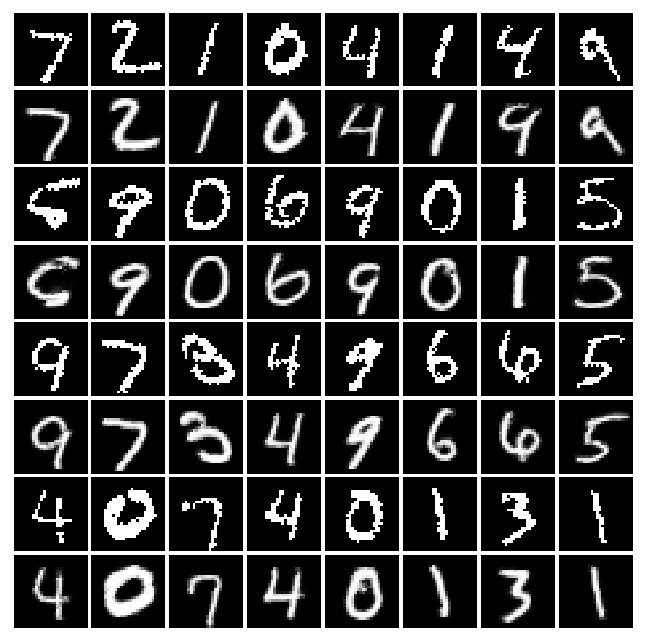
\includegraphics[width=0.22\columnwidth]{images/vae-as-mim-image/2019-08-24_13-22-10_dynamic_mnist_pixelhvae_2level_standard__K_500__wu_100__z1_40_z2_40/real_recon.png}
%     & 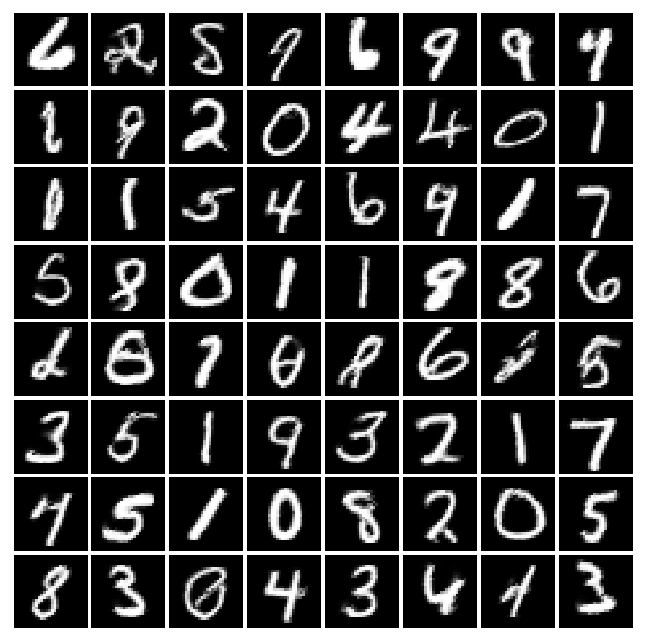
\includegraphics[width=0.22\columnwidth]{images/vae-as-mim-image/2019-08-24_13-22-10_dynamic_mnist_pixelhvae_2level_standard__K_500__wu_100__z1_40_z2_40/generations.png}
%     & 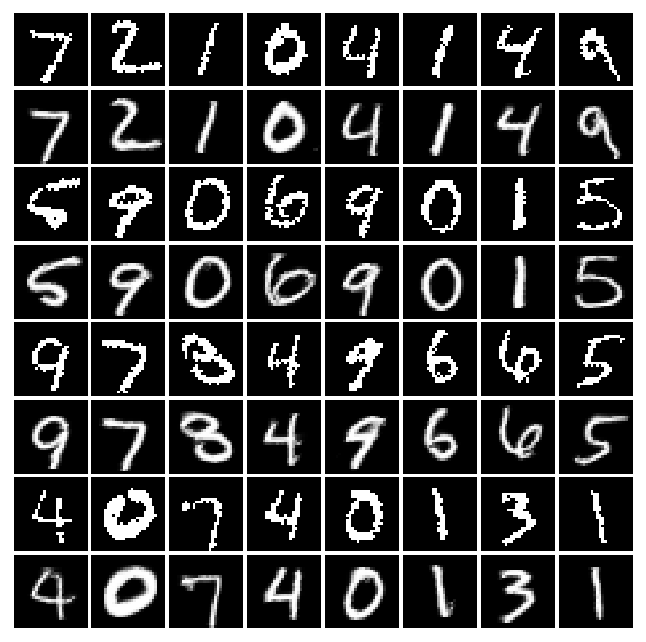
\includegraphics[width=0.22\columnwidth]{images/vae-as-mim-image/2019-08-24_13-22-10_dynamic_mnist_pixelhvae_2level_vampprior__K_500__wu_100__z1_40_z2_40/real_recon.png}
%     & 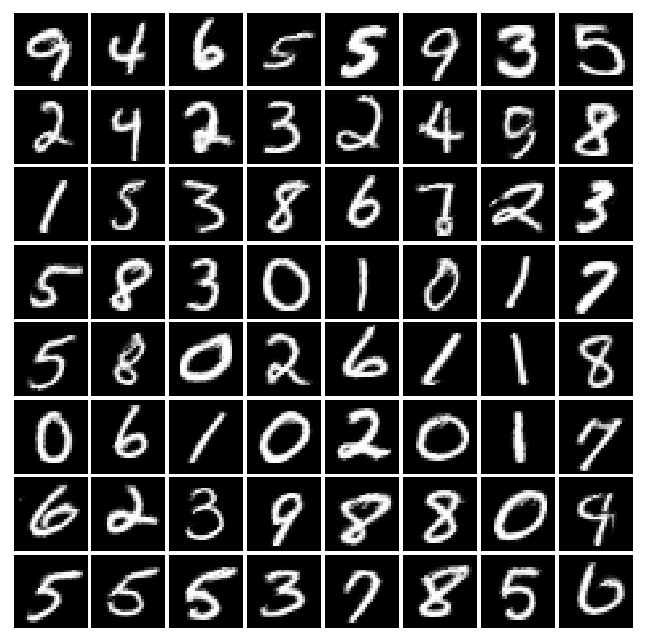
\includegraphics[width=0.22\columnwidth]{images/vae-as-mim-image/2019-08-24_13-22-10_dynamic_mnist_pixelhvae_2level_vampprior__K_500__wu_100__z1_40_z2_40/generations.png}
%     \\
%     {(ii) A-MIM}
%     & 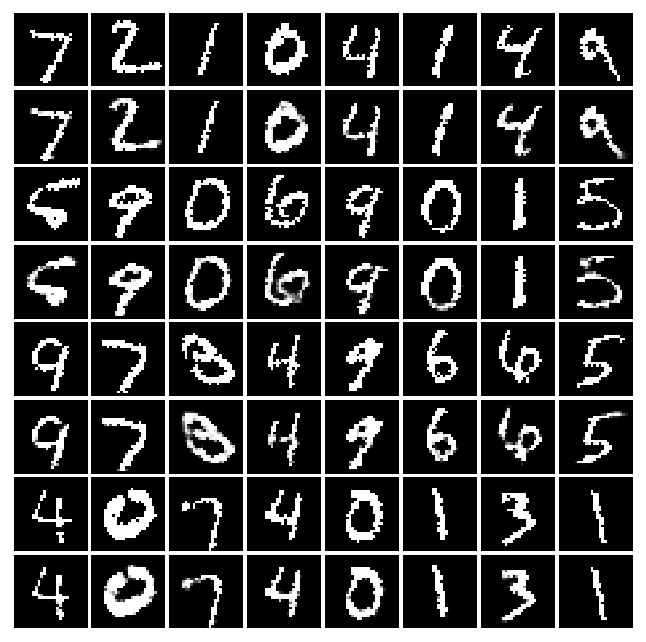
\includegraphics[width=0.22\columnwidth]{images/vae-as-mim-image/2019-08-24_11-48-11_dynamic_mnist_pixelhvae_2level-amim_standard__K_500__wu_100__z1_40_z2_40/real_recon.png}
%     & 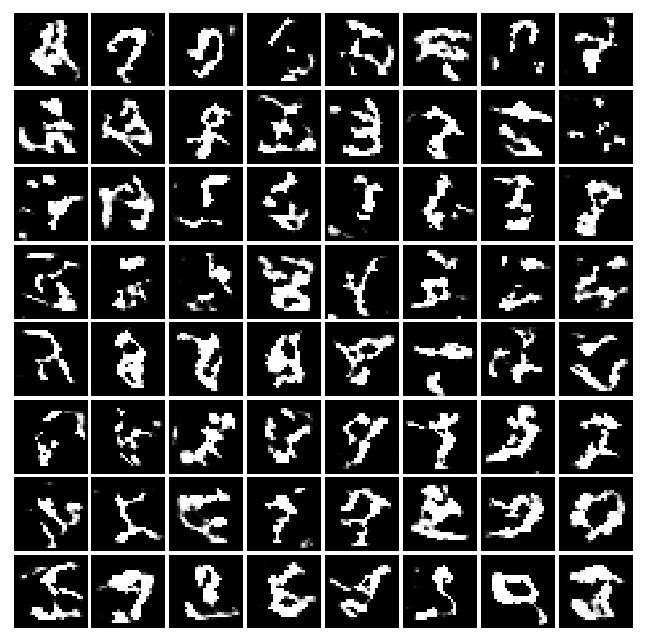
\includegraphics[width=0.22\columnwidth]{images/vae-as-mim-image/2019-08-24_11-48-11_dynamic_mnist_pixelhvae_2level-amim_standard__K_500__wu_100__z1_40_z2_40/generations.png}
%     & 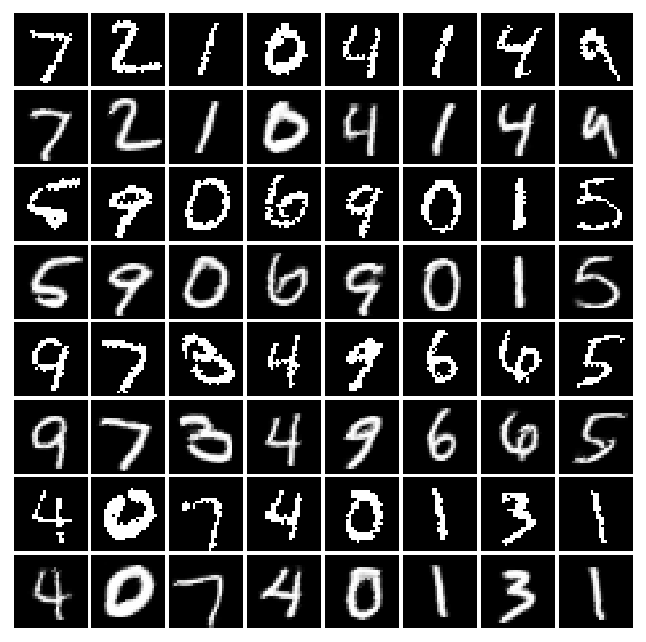
\includegraphics[width=0.22\columnwidth]{images/vae-as-mim-image/2019-08-24_11-48-10_dynamic_mnist_pixelhvae_2level-amim_vampprior__K_500__wu_100__z1_40_z2_40/real_recon.png}
%     & 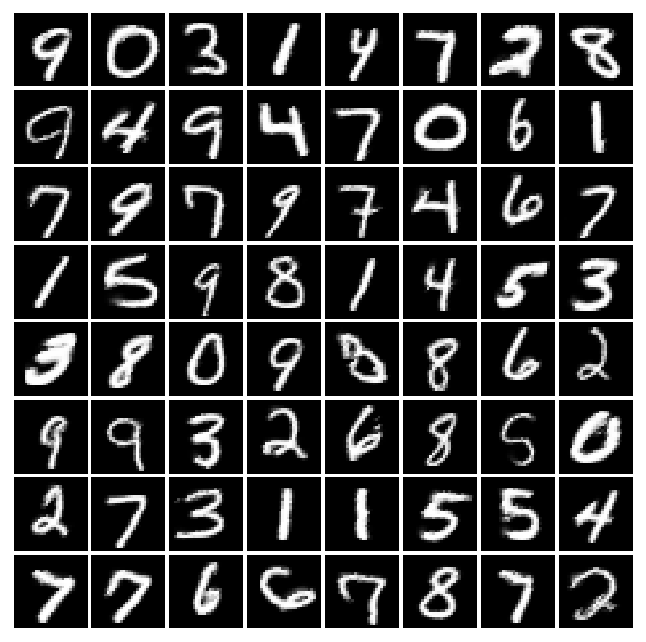
\includegraphics[width=0.22\columnwidth]{images/vae-as-mim-image/2019-08-24_11-48-10_dynamic_mnist_pixelhvae_2level-amim_vampprior__K_500__wu_100__z1_40_z2_40/generations.png}
%     \\
%     & (a) Reconstruction & (b) Model Samples & (c) Reconstruction & (d) Model Samples
%     \end{tabular}
%     \caption{MIM and VAE learning with PixelHVAE (L = 2) for MNIST dataset.}
%     \label{fig:mim-vs-vae-image-qualitative-fasion-mnist}
% \end{figure}


% \begin{figure}[t]
%     \centering
%     \setlength{\tabcolsep}{0pt}
%     \begin{tabular}{m{0.12\textwidth} *4{>{\centering\arraybackslash}m{0.22\textwidth}}}
%     & \multicolumn{2}{c}{Standard Prior} & \multicolumn{2}{c}{VampPrior Prior} \\
%     {(i) VAE}
%     & 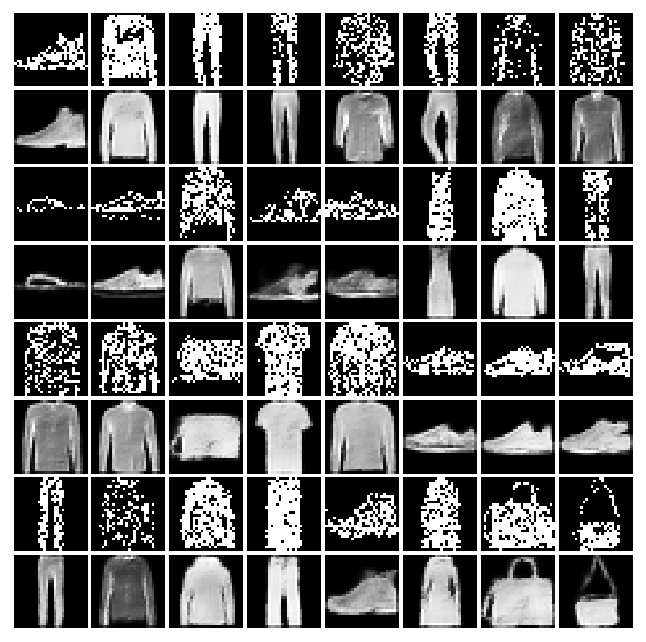
\includegraphics[width=0.22\columnwidth]{images/vae-as-mim-image/2019-08-24_13-22-13_dynamic_fashion_mnist_pixelhvae_2level_standard__K_500__wu_100__z1_40_z2_40/real_recon.png}
%     & 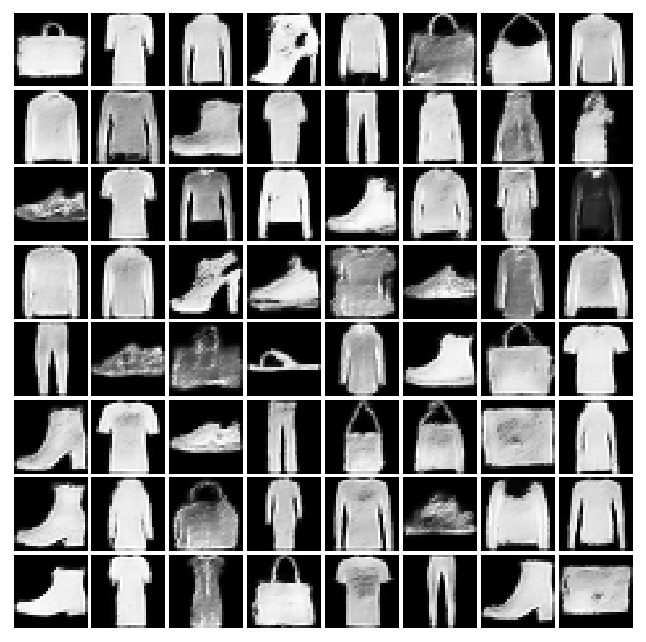
\includegraphics[width=0.22\columnwidth]{images/vae-as-mim-image/2019-08-24_13-22-13_dynamic_fashion_mnist_pixelhvae_2level_standard__K_500__wu_100__z1_40_z2_40/generations.png}
%     & 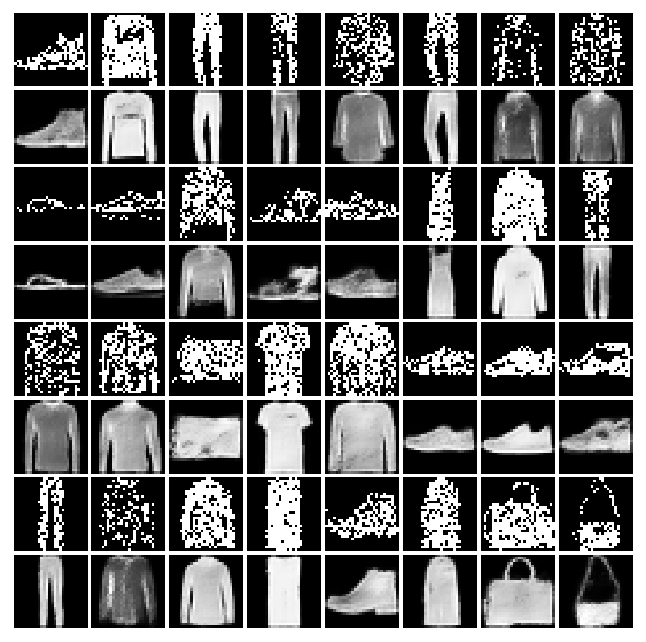
\includegraphics[width=0.22\columnwidth]{images/vae-as-mim-image/2019-08-24_13-22-11_dynamic_fashion_mnist_pixelhvae_2level_vampprior__K_500__wu_100__z1_40_z2_40/real_recon.png}
%     & 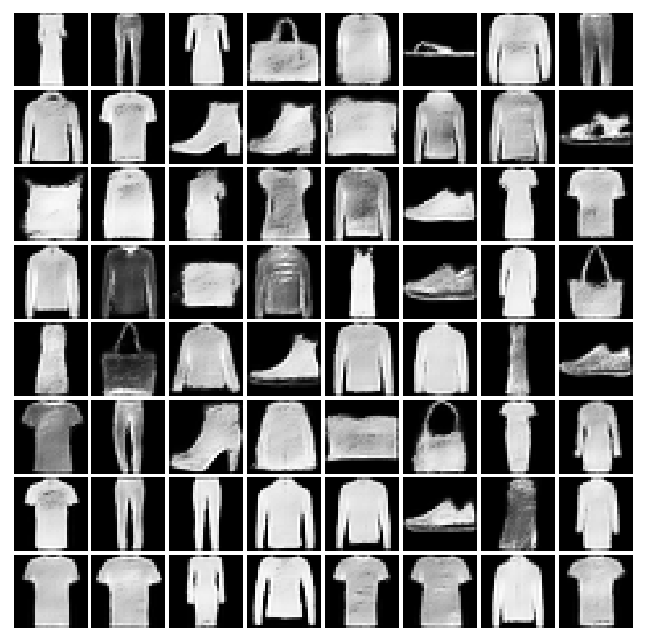
\includegraphics[width=0.22\columnwidth]{images/vae-as-mim-image/2019-08-24_13-22-11_dynamic_fashion_mnist_pixelhvae_2level_vampprior__K_500__wu_100__z1_40_z2_40/generations.png}
%     \\
%     {(ii) A-MIM}
%     & 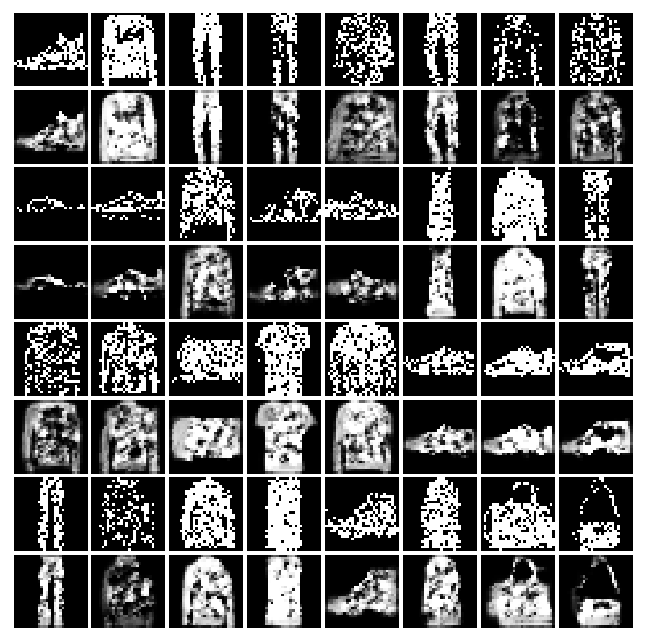
\includegraphics[width=0.22\columnwidth]{images/vae-as-mim-image/2019-08-26_15-47-28_dynamic_fashion_mnist_pixelhvae_2level-amim_standard__K_500__wu_100__z1_40_z2_40/real_recon.png}
%     & 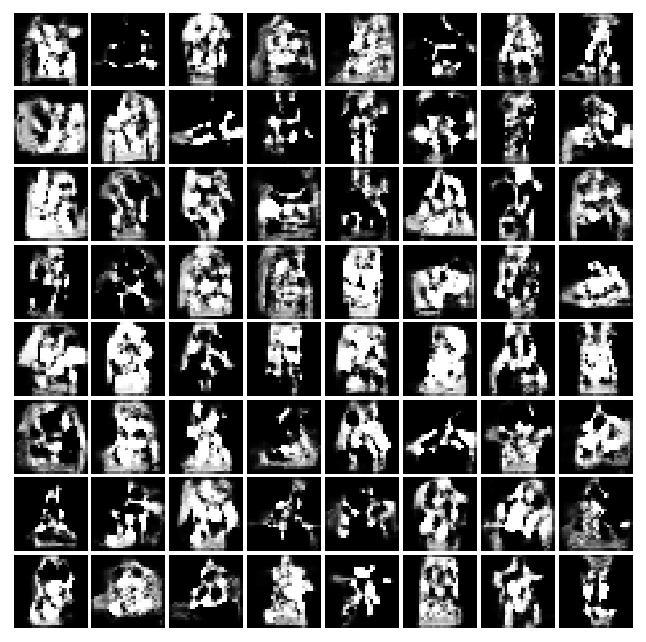
\includegraphics[width=0.22\columnwidth]{images/vae-as-mim-image/2019-08-26_15-47-28_dynamic_fashion_mnist_pixelhvae_2level-amim_standard__K_500__wu_100__z1_40_z2_40/generations.png}
%     & 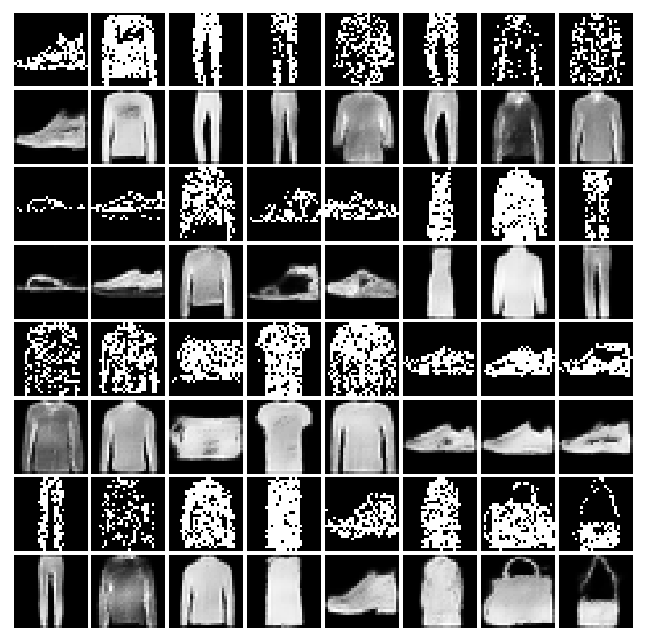
\includegraphics[width=0.22\columnwidth]{images/vae-as-mim-image/2019-08-24_11-48-12_dynamic_fashion_mnist_pixelhvae_2level-amim_vampprior__K_500__wu_100__z1_40_z2_40/real_recon.png}
%     & 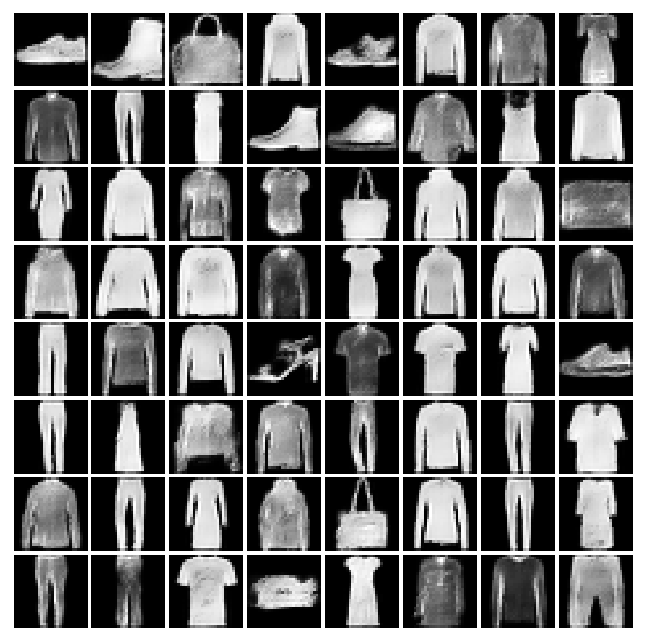
\includegraphics[width=0.22\columnwidth]{images/vae-as-mim-image/2019-08-24_11-48-12_dynamic_fashion_mnist_pixelhvae_2level-amim_vampprior__K_500__wu_100__z1_40_z2_40/generations.png}
%     \\
%     & (a) Reconstruction & (b) Model Samples & (c) Reconstruction & (d) Model Samples
%     \end{tabular}
%     \caption{MIM and VAE learning with PixelHVAE (L = 2) for Fashion MNIST dataset.}
%     \label{fig:mim-vs-vae-image-qualitative-fashion-mnist}
% \end{figure}


% \begin{figure}[t]
%     \centering
%     \setlength{\tabcolsep}{0pt}
%     \begin{tabular}{m{0.12\textwidth} *4{>{\centering\arraybackslash}m{0.22\textwidth}}}
%     & \multicolumn{2}{c}{Standard Prior} & \multicolumn{2}{c}{VampPrior Prior} \\
%     {(i) VAE}
%     & 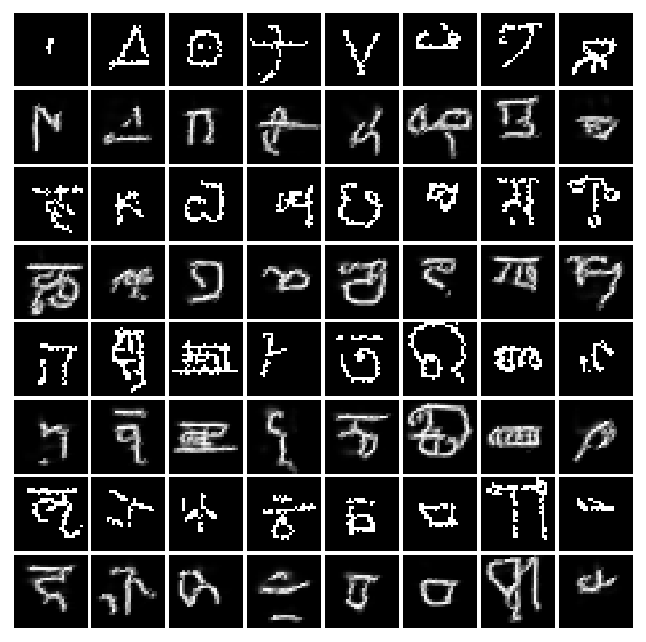
\includegraphics[width=0.22\columnwidth]{images/vae-as-mim-image/2019-08-24_13-22-14_omniglot_pixelhvae_2level_standard__K_500__wu_100__z1_40_z2_40/real_recon.png}
%     & 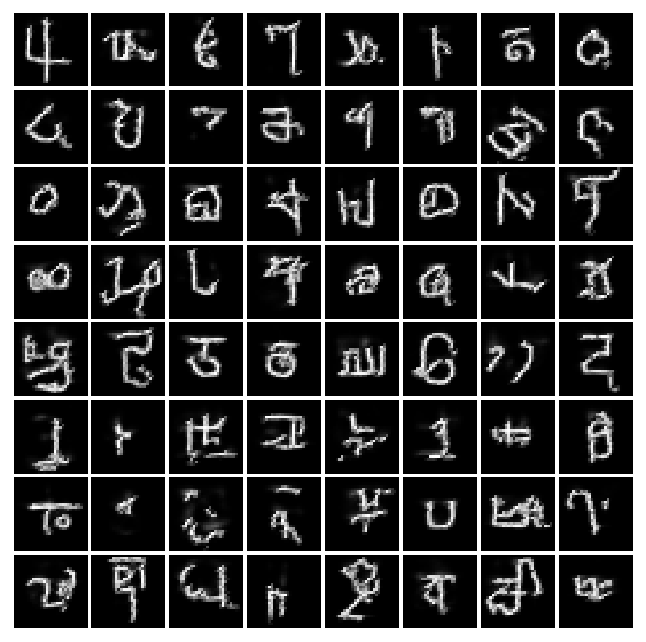
\includegraphics[width=0.22\columnwidth]{images/vae-as-mim-image/2019-08-24_13-22-14_omniglot_pixelhvae_2level_standard__K_500__wu_100__z1_40_z2_40/generations.png}
%     & 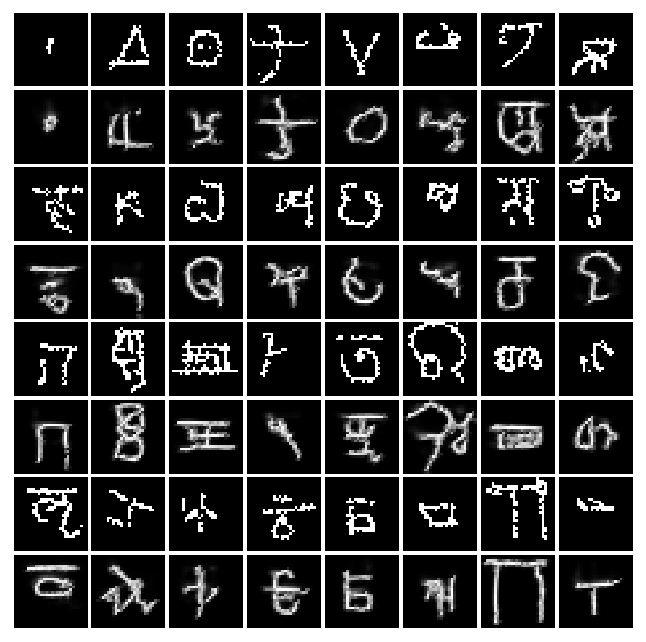
\includegraphics[width=0.22\columnwidth]{images/vae-as-mim-image/2019-08-24_13-22-13_omniglot_pixelhvae_2level_vampprior__K_500__wu_100__z1_40_z2_40/real_recon.png}
%     & 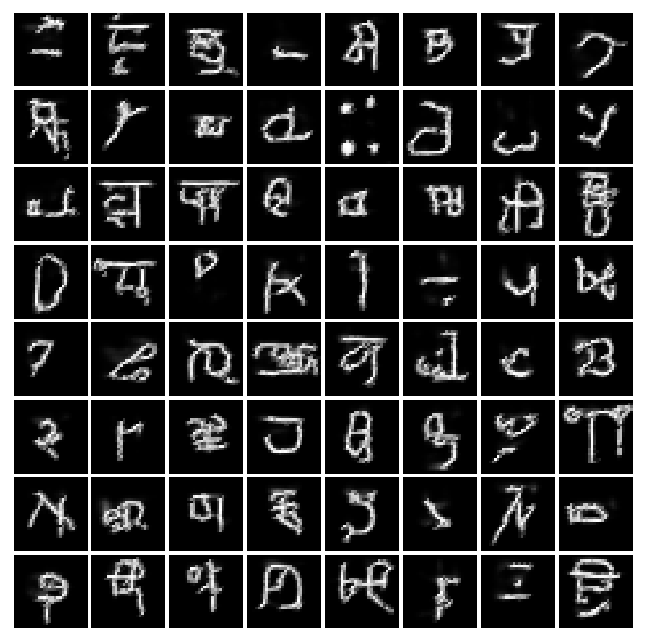
\includegraphics[width=0.22\columnwidth]{images/vae-as-mim-image/2019-08-24_13-22-13_omniglot_pixelhvae_2level_vampprior__K_500__wu_100__z1_40_z2_40/generations.png}
%     \\
%     {(ii) A-MIM}
%     & 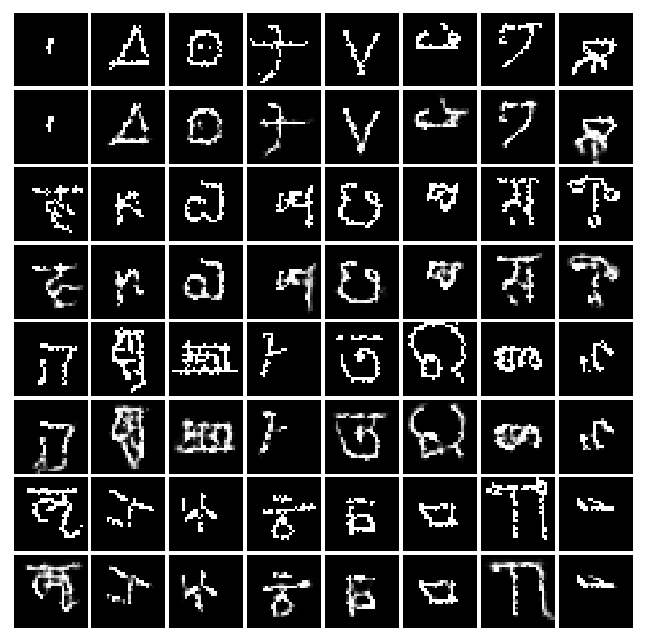
\includegraphics[width=0.22\columnwidth]{images/vae-as-mim-image/2019-08-24_11-48-16_omniglot_pixelhvae_2level-amim_standard__K_500__wu_100__z1_40_z2_40/real_recon.png}
%     & 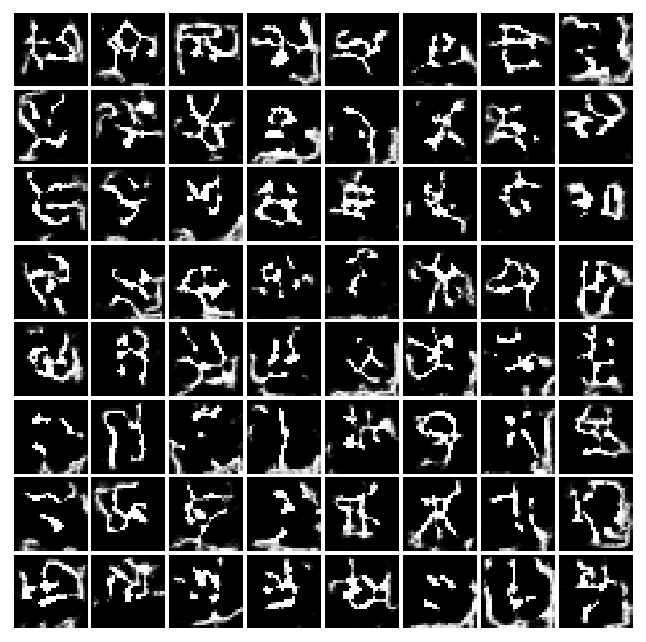
\includegraphics[width=0.22\columnwidth]{images/vae-as-mim-image/2019-08-24_11-48-16_omniglot_pixelhvae_2level-amim_standard__K_500__wu_100__z1_40_z2_40/generations.png}
%     & 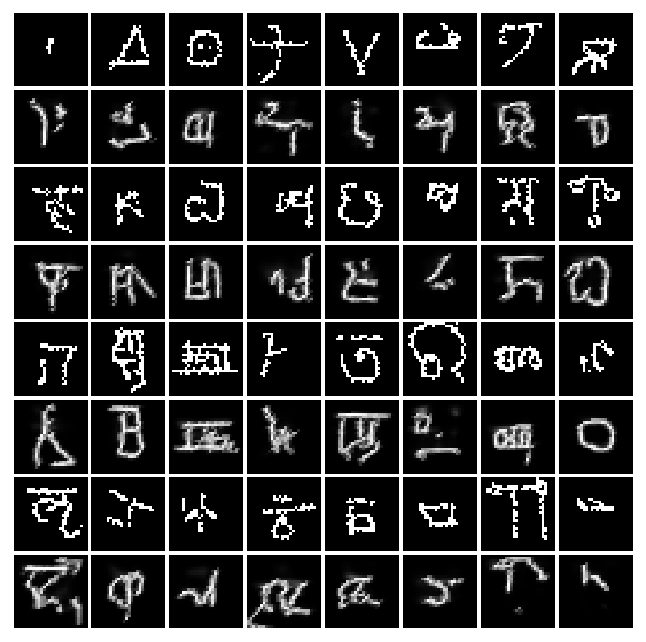
\includegraphics[width=0.22\columnwidth]{images/vae-as-mim-image/2019-08-24_11-48-14_omniglot_pixelhvae_2level-amim_vampprior__K_500__wu_100__z1_40_z2_40/real_recon.png}
%     & 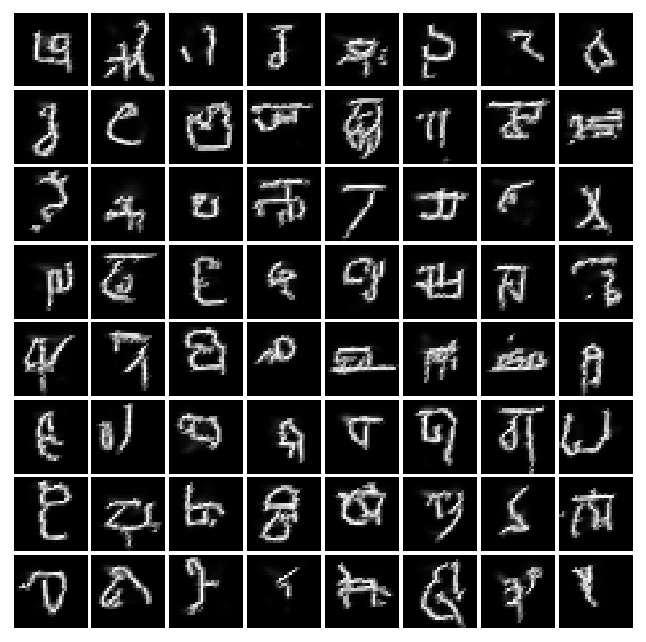
\includegraphics[width=0.22\columnwidth]{images/vae-as-mim-image/2019-08-24_11-48-14_omniglot_pixelhvae_2level-amim_vampprior__K_500__wu_100__z1_40_z2_40/generations.png}
%     \\
%     & (a) Reconstruction & (b) Model Samples & (c) Reconstruction & (d) Model Samples
%     \end{tabular}
%     \caption{MIM and VAE learning with PixelHVAE (L = 2) for Omniglot dataset.}
%     \label{fig:mim-vs-vae-image-qualitative-omniglot}
% \end{figure}

% \begin{table}[t]
%     \centering
%     \setlength{\tabcolsep}{0.5em} % for the horizontal padding
%     {
%     %\tiny
%     \footnotesize
%     \renewcommand{\arraystretch}{1.2}% for the vertical padding
%     \begin{tabular}{l||c|c|c||c|c|c||c|c||c|c||}
%          \multicolumn{1}{l||}{} &  \multicolumn{3}{c||}{convHVAE (L = 2) S}  & \multicolumn{3}{c||}{convHVAE (L = 2) VP}  & \multicolumn{2}{c||}{PixelHVAE (L = 2) S}  & \multicolumn{2}{c||}{PixelHVAE (L = 2) VP} \\
%          Dataset & {\tiny MIM} & {\tiny A-MIM} & {\tiny VAE} & {\tiny MIM} & {\tiny A-MIM} & {\tiny VAE} & {\tiny A-MIM} & {\tiny VAE} & {\tiny A-MIM} & {\tiny VAE}  \\
%         \hline
%         Fashion MNIST & -291.82 & -263.13 & \textbf{-225.43} & -253.34 & -226 & \textbf{-224.86} & -243.8 & -224.68 & -224.86 & \textbf{-223.97} \\
%         MNIST         & -142.31 & -123.85 & \textbf{-80.56} & -106.26 & -80.51 & \textbf{-79.79}  & -113.59 & -78.83 & -78.96 & \textbf{-78.57} \\
%         Omniglot      & -158.96 & -140.7 & \textbf{-98.29} & -108.95  & -100.56 & \textbf{-97.38}  & -125.56 & -90.96 & -92.11 & \textbf{-90.79} \\
%     \end{tabular}
%     }
%     \vspace*{0.5cm}
%     \caption{Test log-likelihood (LL) for MIM learning and VAE learning (higher is better) See text for details.
%     \david{do we neeed A-MIM and MIM for models where MIM was possible?}
%     }
%     \label{tab:mim-vs-vae-image-quantitative-ll}
% \end{table}

\begin{table}[t]
    \centering
    \setlength{\tabcolsep}{0.5em} % for the horizontal padding
    {
    % \tiny
    \scriptsize
    % \footnotesize
    \renewcommand{\arraystretch}{1.2}% for the vertical padding
    \begin{tabular}{l||c|c||c|c||c|c||c|c||}
         \multicolumn{1}{l||}{} &  \multicolumn{2}{c||}{convHVAE (L = 2) S}  & \multicolumn{2}{c||}{convHVAE (L = 2) VP}  & \multicolumn{2}{c||}{PixelHVAE (L = 2) S}  & \multicolumn{2}{c||}{PixelHVAE (L = 2) VP} \\
         Dataset & {\tiny MIM} &  {\tiny VAE} & {\tiny MIM}  & {\tiny VAE} & {\tiny A-MIM} & {\tiny VAE} & {\tiny A-MIM} & {\tiny VAE}  \\
        \hline
        Fashion MNIST & -291.82 &  \textbf{-225.43} & -253.34 & \textbf{-224.86} & -243.8 & \textbf{-224.68} & -224.86 & \textbf{-223.97} \\
        MNIST         & -142.31 &  \textbf{-80.56} & -106.26 &  \textbf{-79.79}  & -113.59 & \textbf{-78.83} & -78.96 & \textbf{-78.57} \\
        Omniglot      & -158.96 &  \textbf{-98.29} & -108.95 & \textbf{-97.38}  & -125.56 & \textbf{-90.96} & -92.11 & \textbf{-90.79} \\
    \end{tabular}
    }
    \vspace*{0.5cm}
    \caption{Test log-likelihood (LL) for MIM learning and VAE learning (higher is better) See text for details.
    }
    \label{tab:mim-vs-vae-image-quantitative-ll}
\end{table}


\begin{figure}[t]
    \centering
    \setlength{\tabcolsep}{0pt}
    \begin{tabular}{*4{>{\centering\arraybackslash}m{0.25\textwidth}}}
    \multicolumn{2}{c}{Standard Prior} & \multicolumn{2}{c}{VampPrior Prior} \\
    \multicolumn{2}{c}{\includegraphics[width=0.5\columnwidth]{images/vae-as-mim-image/2019-08-24_13-22-13_dynamic_fashion_mnist_pixelhvae_2level_standard__K_500__wu_100__z1_40_z2_40/real_flat.png}} 
    & \multicolumn{2}{c}{\includegraphics[width=0.5\columnwidth]{images/vae-as-mim-image/2019-08-24_13-22-11_dynamic_fashion_mnist_pixelhvae_2level_vampprior__K_500__wu_100__z1_40_z2_40/real_flat.png}} 
    \\[-0.2cm]
    \multicolumn{2}{c}{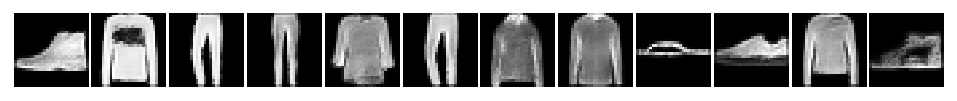
\includegraphics[width=0.5\columnwidth]{images/vae-as-mim-image/2019-08-24_13-22-13_dynamic_fashion_mnist_pixelhvae_2level_standard__K_500__wu_100__z1_40_z2_40/reconstructions_flat.png}} 
    & \multicolumn{2}{c}{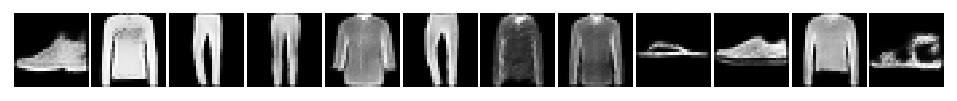
\includegraphics[width=0.5\columnwidth]{images/vae-as-mim-image/2019-08-24_13-22-11_dynamic_fashion_mnist_pixelhvae_2level_vampprior__K_500__wu_100__z1_40_z2_40/reconstructions_flat.png}} 
    \\[-0.2cm]
    \multicolumn{2}{c}{\includegraphics[width=0.5\columnwidth]{images/vae-as-mim-image/2019-08-26_15-47-28_dynamic_fashion_mnist_pixelhvae_2level-amim_standard__K_500__wu_100__z1_40_z2_40/reconstructions_flat.png}} 
    & \multicolumn{2}{c}{\includegraphics[width=0.5\columnwidth]{images/vae-as-mim-image/2019-08-24_11-48-12_dynamic_fashion_mnist_pixelhvae_2level-amim_vampprior__K_500__wu_100__z1_40_z2_40/reconstructions_flat.png}} 
    \\
    \includegraphics[width=0.25\columnwidth]{images/vae-as-mim-image/2019-08-24_13-22-13_dynamic_fashion_mnist_pixelhvae_2level_standard__K_500__wu_100__z1_40_z2_40/generations.png}
    & \includegraphics[width=0.25\columnwidth]{images/vae-as-mim-image/2019-08-26_15-47-28_dynamic_fashion_mnist_pixelhvae_2level-amim_standard__K_500__wu_100__z1_40_z2_40/generations.png}
    & \includegraphics[width=0.25\columnwidth]{images/vae-as-mim-image/2019-08-24_13-22-11_dynamic_fashion_mnist_pixelhvae_2level_vampprior__K_500__wu_100__z1_40_z2_40/generations.png}
    & \includegraphics[width=0.25\columnwidth]{images/vae-as-mim-image/2019-08-24_11-48-12_dynamic_fashion_mnist_pixelhvae_2level-amim_vampprior__K_500__wu_100__z1_40_z2_40/generations.png}
    \\
    (a) VAE (S) & (b) A-MIM (S) & (c) VAE (VP) & (d) A-MIM (VP)
    \end{tabular}
    \caption{MIM and VAE learning with PixelHVAE (L = 2) for Fashion MNIST dataset. Top three rows are data samples, VAE, A-MIM, correspondingly. Bottom row is model samples.}
    \label{fig:mim-vs-vae-image-qualitative-fashion-mnist}
\end{figure}

\begin{figure}[t]
    \centering
    \setlength{\tabcolsep}{0pt}
    \begin{tabular}{*4{>{\centering\arraybackslash}m{0.25\textwidth}}}
    \multicolumn{2}{c}{Standard Prior} & \multicolumn{2}{c}{VampPrior Prior} \\
    \multicolumn{2}{c}{\includegraphics[width=0.5\columnwidth]{images/vae-as-mim-image/2019-08-24_13-22-10_dynamic_mnist_pixelhvae_2level_standard__K_500__wu_100__z1_40_z2_40/real_flat.png}} 
    & \multicolumn{2}{c}{\includegraphics[width=0.5\columnwidth]{images/vae-as-mim-image/2019-08-24_13-22-10_dynamic_mnist_pixelhvae_2level_vampprior__K_500__wu_100__z1_40_z2_40/real_flat.png}} 
    \\[-0.2cm]
    \multicolumn{2}{c}{\includegraphics[width=0.5\columnwidth]{images/vae-as-mim-image/2019-08-24_13-22-10_dynamic_mnist_pixelhvae_2level_standard__K_500__wu_100__z1_40_z2_40/reconstructions_flat.png}} 
    & \multicolumn{2}{c}{\includegraphics[width=0.5\columnwidth]{images/vae-as-mim-image/2019-08-24_13-22-10_dynamic_mnist_pixelhvae_2level_vampprior__K_500__wu_100__z1_40_z2_40/reconstructions_flat.png}} 
    \\[-0.2cm]
    \multicolumn{2}{c}{\includegraphics[width=0.5\columnwidth]{images/vae-as-mim-image/2019-08-24_11-48-11_dynamic_mnist_pixelhvae_2level-amim_standard__K_500__wu_100__z1_40_z2_40/reconstructions_flat.png}} 
    & \multicolumn{2}{c}{\includegraphics[width=0.5\columnwidth]{images/vae-as-mim-image/2019-08-24_11-48-10_dynamic_mnist_pixelhvae_2level-amim_vampprior__K_500__wu_100__z1_40_z2_40/reconstructions_flat.png}} 
    \\
    \includegraphics[width=0.25\columnwidth]{images/vae-as-mim-image/2019-08-24_13-22-10_dynamic_mnist_pixelhvae_2level_standard__K_500__wu_100__z1_40_z2_40/generations.png}
    & \includegraphics[width=0.25\columnwidth]{images/vae-as-mim-image/2019-08-24_11-48-11_dynamic_mnist_pixelhvae_2level-amim_standard__K_500__wu_100__z1_40_z2_40/generations.png}
    & \includegraphics[width=0.25\columnwidth]{images/vae-as-mim-image/2019-08-24_13-22-10_dynamic_mnist_pixelhvae_2level_vampprior__K_500__wu_100__z1_40_z2_40/generations.png}
    & \includegraphics[width=0.25\columnwidth]{images/vae-as-mim-image/2019-08-24_11-48-10_dynamic_mnist_pixelhvae_2level-amim_vampprior__K_500__wu_100__z1_40_z2_40/generations.png}
    \\
    (a) VAE (S) & (b) A-MIM (S) & (c) VAE (VP) & (d) A-MIM (VP)
    \end{tabular}
    \caption{MIM and VAE learning with PixelHVAE (L = 2) for MNIST dataset. Top three rows are data samples, VAE, A-MIM, correspondingly. Bottom row is model samples.}
    \label{fig:mim-vs-vae-image-qualitative-mnist}
\end{figure}

\begin{figure}[t]
    \centering
    \setlength{\tabcolsep}{0pt}
    \begin{tabular}{*4{>{\centering\arraybackslash}m{0.25\textwidth}}}
    \multicolumn{2}{c}{Standard Prior} & \multicolumn{2}{c}{VampPrior Prior} \\
    \multicolumn{2}{c}{\includegraphics[width=0.5\columnwidth]{images/vae-as-mim-image/2019-08-24_13-22-14_omniglot_pixelhvae_2level_standard__K_500__wu_100__z1_40_z2_40/real_flat.png}} 
    & \multicolumn{2}{c}{\includegraphics[width=0.5\columnwidth]{images/vae-as-mim-image/2019-08-24_13-22-13_omniglot_pixelhvae_2level_vampprior__K_500__wu_100__z1_40_z2_40/real_flat.png}} 
    \\[-0.2cm]
    \multicolumn{2}{c}{\includegraphics[width=0.5\columnwidth]{images/vae-as-mim-image/2019-08-24_13-22-14_omniglot_pixelhvae_2level_standard__K_500__wu_100__z1_40_z2_40/reconstructions_flat.png}} 
    & \multicolumn{2}{c}{\includegraphics[width=0.5\columnwidth]{images/vae-as-mim-image/2019-08-24_13-22-13_omniglot_pixelhvae_2level_vampprior__K_500__wu_100__z1_40_z2_40/reconstructions_flat.png}} 
    \\[-0.2cm]
    \multicolumn{2}{c}{\includegraphics[width=0.5\columnwidth]{images/vae-as-mim-image/2019-08-24_11-48-16_omniglot_pixelhvae_2level-amim_standard__K_500__wu_100__z1_40_z2_40/reconstructions_flat.png}} 
    & \multicolumn{2}{c}{\includegraphics[width=0.5\columnwidth]{images/vae-as-mim-image/2019-08-24_11-48-14_omniglot_pixelhvae_2level-amim_vampprior__K_500__wu_100__z1_40_z2_40/reconstructions_flat.png}} 
    \\
    \includegraphics[width=0.25\columnwidth]{images/vae-as-mim-image/2019-08-24_13-22-14_omniglot_pixelhvae_2level_standard__K_500__wu_100__z1_40_z2_40/generations.png}
    & \includegraphics[width=0.25\columnwidth]{images/vae-as-mim-image/2019-08-24_11-48-16_omniglot_pixelhvae_2level-amim_standard__K_500__wu_100__z1_40_z2_40/generations.png}
    & \includegraphics[width=0.25\columnwidth]{images/vae-as-mim-image/2019-08-24_13-22-13_omniglot_pixelhvae_2level_vampprior__K_500__wu_100__z1_40_z2_40/generations.png}
    & \includegraphics[width=0.25\columnwidth]{images/vae-as-mim-image/2019-08-24_11-48-14_omniglot_pixelhvae_2level-amim_vampprior__K_500__wu_100__z1_40_z2_40/generations.png}
    \\
    (a) VAE (S) & (b) A-MIM (S) & (c) VAE (VP) & (d) A-MIM (VP)
    \end{tabular}
    \caption{MIM and VAE learning with PixelHVAE (L = 2) for Omniglot dataset. Top three rows are data samples, VAE, A-MIM, correspondingly. Bottom row is model samples.}
    \label{fig:mim-vs-vae-image-qualitative-omniglot}
\end{figure}


% \david{Expt goal to show learning on higher dimensional image data.
% Here we don't try to compute MI since the results are not reliable.
% Instead we focus on reconstructions and random samples for evaluation.
% We also show different architectures at play. etc.}
% \david{We need to discuss why A-MIM is used (ie cost of AR model for generation.}
% \david{Explain architectures used incl priors like vamp prior if this is where it is 
% first introduced.}
% \david{What should plots show:  Shows cases in which VAE reconstructions were 
% clearly wrong but the MIM reconstructions were correct. show a couple of those.}

Here we explore learning on higher dimensional image data, where we cannot directly compute mutual information since the results are not reliable \cite{Hjelm2018}. Instead we focus on log-likelihood, reconstructions, and random samples for evaluation. We experiment with MNIST \cite{LeCun1998}, Fashion MNIST \cite{DBLP:journals/corr/abs-1708-07747}, and Omniglot \cite{Lake2015} datasets.
In what follows we explore multiple architectures of VAE models, and the corresponding MIM models (see Algorithm.\ \ref{algo:vae-as-mim}), where we use VAE as the baseline for comparison.

We experiment with the top performing models from \cite{DBLP:journals/corr/TomczakW17}, namely: convHVAE (L = 2) and PixelHVAE (L = 2), with Standard (S) priors which are the usual Normal distributions, and VampPrior (VP) priors which define the prior as a mixture model of the encoder conditioned on learnable pseudo-inputs $\bs{u}_k$, or explicitly $\Mdec(\z) = \frac{1}{K}\sum_{k=1}^{K} \Menc(\z|\bs{u}_k)$. In all the experiments we used the same setup that was used in \cite{DBLP:journals/corr/TomczakW17}, and with the same latent dimensionality $\z \in \mathbb{R}^{80}$. By doing so we aim to highlight the generality of MIM learning as being architecture independent, and to provide examples for the training procedure of existing VAE architectures with MIM learning. 

We show quantitative results in Table\ \ref{tab:mim-vs-vae-image-quantitative-ll} for test log-likelihood,
which shows that VAE models results in better log-likelihood (LL), but with a rather small gap for the more expressive models (\ie, PixelHVAE (L = 2) with VampPrior). Following \cite{DBLP:journals/corr/TomczakW17} we omit the standard deviation from the table, being no larger than 0.03. We also show qualitative results for the most expressive models (\ie, PixelHVAE). Figures\ (\ref{fig:mim-vs-vae-image-qualitative-fashion-mnist}, \ref{fig:mim-vs-vae-image-qualitative-mnist}, \ref{fig:mim-vs-vae-image-qualitative-omniglot}), depict reconstruction, and sampling for Fashion-MNIST, MNIST, and Omniglot, correspondingly.
The top three rows of each of the plots depicts data samples, VAE reconstruction, and A-MIM reconstruction, respectively. The bottom row depicts samples. We point that while MIM with a weak prior (Standard) presents better reconstruction than VAE, it suffers from poor sampling (b). Increasing the expressiveness results in comparable samples and reconstruction.
The poor sampling with a weak prior can be explained by the tightly clustered latent representation (\eg, Fig.\ \ref{fig:posterior-collapse-qualitative}). An expressive learnable prior can learn those clusters, and as such produces good samples.
In other words, while VAE opt for better sampling on the expense of lower mutual information, MIM targets higher mutual information on the expense of worse sampling. In Sec.\ \ref{sec:representation-learning-with-mim} we probe the effect of higher mutual information on the quality of the learned representation.
%  We conclude that MIM fully utilizes the more powerful model, and given expressive enough model will provide same or better results, when comared to VAE.


%%%%%%%%%%%%%%%%%%%%%%%%%%%%%%%%%%%%%%%%%%%%%%%%%%%%%%%%
\subsection{Representation Learning with MIM} 
\label{sec:representation-learning-with-mim}

% \begin{table}[t]
%     \centering
%     \setlength{\tabcolsep}{0.5em} % for the horizontal padding
%     {
%     % \tiny
%     \footnotesize
%     \renewcommand{\arraystretch}{1.2}% for the vertical padding
%     \begin{tabular}{l||c|c|c||c|c|c||c|c||c|c||}
%          \multicolumn{1}{l||}{} &  \multicolumn{3}{c||}{convHVAE (L = 2) S}  & \multicolumn{3}{c||}{convHVAE (L = 2) VP}  & \multicolumn{2}{c||}{PixelHVAE (L = 2) S}  & \multicolumn{2}{c||}{PixelHVAE (L = 2) VP} \\
%          Dataset & {\tiny MIM} & {\tiny A-MIM} & {\tiny VAE} & {\tiny MIM} & {\tiny A-MIM} & {\tiny VAE} & {\tiny A-MIM} & {\tiny VAE} & {\tiny A-MIM} & {\tiny VAE}  \\
%         \hline
%         Fashion MNIST & \textbf{11266.17} & 10726.26 & 2043.2 & \textbf{7035.3} & 2038.62 & 2061.36 & \textbf{11251.16}  & 1114.26 & 1173.17 & \textbf{1223.07}  \\
%         MNIST         & \textbf{11618.63} & 10532.9 & 2674.42 & \textbf{7274.62} & 2636.59 & 2625.34 & \textbf{10667} & 1270.08 & 1252.37 & \textbf{1340.93} \\
%         Omniglot      &  \textbf{9340.47} & 8473.475 & 3212.76 & \textbf{4161.87} & 2996.8 & 3159.76 & \textbf{8656.52} & 676.0 & 515.7 & \textbf{641.56}  \\
%     \end{tabular}
%     }
%     \vspace*{0.5cm}
%     \caption{Test mutual information for MIM learning and VAE learning (higher is better). See text for details.\micha{train A-MIM PixelCNN + VP to prevent overfitting, or train MIM for that case}}
%     \label{tab:mim-vs-vae-image-quantitative-mi}
% \end{table}

% \begin{table}[t]
%     \centering
%     \setlength{\tabcolsep}{0.5em} % for the horizontal padding
%     {
%     % \tiny
%     \footnotesize
%     \renewcommand{\arraystretch}{1.2}% for the vertical padding
%     \begin{tabular}{l||c|c|c||c|c|c||c|c||c|c||}
%          \multicolumn{1}{l||}{} &  \multicolumn{3}{c||}{convHVAE (L = 2) S}  & \multicolumn{3}{c||}{convHVAE (L = 2) VP}  & \multicolumn{2}{c||}{PixelHVAE (L = 2) S}  & \multicolumn{2}{c||}{PixelHVAE (L = 2) VP} \\
%          Dataset & {\tiny MIM} & {\tiny A-MIM} & {\tiny VAE} & {\tiny MIM} & {\tiny A-MIM} & {\tiny VAE} & {\tiny A-MIM} & {\tiny VAE} & {\tiny A-MIM} & {\tiny VAE}  \\
%         \hline
%         \multirow{1}{*}{Fashion MNIST}
%         & \textbf{0.84} & 0.82 & 0.75 & \textbf{0.84} & 0.82 & 0.76  & 0.69 & \textbf{0.75} & \textbf{0.8} & 0.74 \\
%         \hline
%         \multirow{1}{*}{MNIST}
%         & \textbf{0.98} & 0.97 & 0.91  & \textbf{0.98}  & \textbf{0.98} & 0.85 & \textbf{0.95} & 0.87 & \textbf{0.97} & 0.85 \\
%     \end{tabular}
%     }
%     \vspace*{0.5cm}
%     \caption{Test classification accuracy of K-NN classifier for MIM learning and VAE learning. MIM and A-MIM consistently cluster classes in the latent representation in an unsupervised manner.}
%     \label{tab:mim-vs-vae-image-quantitative-cls}
% \end{table}

% \begin{figure}[t]
%     \tiny
%     \centering
%     \setlength{\tabcolsep}{0pt}
%     \begin{tabular}{m{0.10\textwidth} *3{>{\centering\arraybackslash}m{0.3\textwidth}}}
%     {(i) S}
%     & \includegraphics[width=0.3\columnwidth]{images/vae-as-mim-image/2019-08-23_03-32-32_dynamic_fashion_mnist_convhvae_2level_standard__K_500__wu_100__z1_40_z2_40/z_embed.png}
%     & \includegraphics[width=0.3\columnwidth]{images/vae-as-mim-image/2019-08-23_03-39-06_dynamic_fashion_mnist_convhvae_2level-amim_standard__K_500__wu_100__z1_40_z2_40/z_embed.png}
%     & \includegraphics[width=0.3\columnwidth]{images/vae-as-mim-image/2019-08-23_03-36-28_dynamic_fashion_mnist_convhvae_2level-smim_standard__K_500__wu_100__z1_40_z2_40/z_embed.png}
%     \\
%     {(ii) VP}
%     & \includegraphics[width=0.3\columnwidth]{images/vae-as-mim-image/2019-08-23_03-23-06_dynamic_fashion_mnist_convhvae_2level_vampprior__K_500__wu_100__z1_40_z2_40/z_embed.png}
%     & \includegraphics[width=0.3\columnwidth]{images/vae-as-mim-image/2019-08-23_03-37-39_dynamic_fashion_mnist_convhvae_2level-amim_vampprior__K_500__wu_100__z1_40_z2_40/z_embed.png}
%     & \includegraphics[width=0.3\columnwidth]{images/vae-as-mim-image/2019-08-23_03-33-22_dynamic_fashion_mnist_convhvae_2level-smim_vampprior__K_500__wu_100__z1_40_z2_40/z_embed.png}
%     \\
%      & VAE & A-MIM  & MIM \\
%     \end{tabular}
%     \caption{MIM and VAE $\z$ embedding for Fashion MNIST with convHVAE (L = 2) architecture.\micha{K=1,3,5,10}}
%     \label{fig:mim-vs-vae-image-z-embed-fashion-mnist}
% \end{figure}

% \begin{figure}[t]
%     \tiny
%     \centering
%     \setlength{\tabcolsep}{0pt}
%     \begin{tabular}{m{0.10\textwidth} *3{>{\centering\arraybackslash}m{0.3\textwidth}}}
%     {(i) S}
%     & \includegraphics[width=0.3\columnwidth]{images/vae-as-mim-image/2019-08-22_19-01-54_dynamic_mnist_convhvae_2level_standard__K_500__wu_100__z1_40_z2_40/z_embed.png}
%     & \includegraphics[width=0.3\columnwidth]{images/vae-as-mim-image/2019-08-22_19-48-18_dynamic_mnist_convhvae_2level-amim_standard__K_500__wu_100__z1_40_z2_40/z_embed.png}
%     & \includegraphics[width=0.3\columnwidth]{images/vae-as-mim-image/2019-08-22_19-12-58_dynamic_mnist_convhvae_2level-smim_standard__K_500__wu_100__z1_40_z2_40/z_embed.png}
%     \\
%     {(ii) VP}
%     & \includegraphics[width=0.3\columnwidth]{images/vae-as-mim-image/2019-08-22_18-59-01_dynamic_mnist_convhvae_2level_vampprior__K_500__wu_100__z1_40_z2_40/z_embed.png}
%     & \includegraphics[width=0.3\columnwidth]{images/vae-as-mim-image/2019-08-22_19-26-50_dynamic_mnist_convhvae_2level-amim_vampprior__K_500__wu_100__z1_40_z2_40/z_embed.png}
%     & \includegraphics[width=0.3\columnwidth]{images/vae-as-mim-image/2019-08-22_19-06-26_dynamic_mnist_convhvae_2level-smim_vampprior__K_500__wu_100__z1_40_z2_40/z_embed.png}
%     \\
%      & VAE & A-MIM  & MIM \\
%     \end{tabular}
%     \caption{MIM and VAE $\z$ embedding for MNIST with convHVAE (L = 2) architecture.}
%     \label{fig:mim-vs-vae-image-z-embed-mnist}
% \end{figure}

% \begin{figure}[t]
%     \tiny
%     \centering
%     \setlength{\tabcolsep}{0pt}
%     \begin{tabular}{m{0.10\textwidth} *4{>{\centering\arraybackslash}m{0.22\textwidth}}}
%     & \multicolumn{2}{c}{MNIST} & \multicolumn{2}{c}{Fashion MNIST} \\
%     {(i) VAE}
%     & \includegraphics[width=0.22\columnwidth]{images/vae-as-mim-image/2019-08-24_13-22-10_dynamic_mnist_pixelhvae_2level_standard__K_500__wu_100__z1_40_z2_40/z_embed.png}
%     & \includegraphics[width=0.22\columnwidth]{images/vae-as-mim-image/2019-08-24_13-22-10_dynamic_mnist_pixelhvae_2level_vampprior__K_500__wu_100__z1_40_z2_40/z_embed.png}
%     & \includegraphics[width=0.22\columnwidth]{images/vae-as-mim-image/2019-08-24_13-22-13_dynamic_fashion_mnist_pixelhvae_2level_standard__K_500__wu_100__z1_40_z2_40/z_embed.png}
%     & \includegraphics[width=0.22\columnwidth]{images/vae-as-mim-image/2019-08-24_13-22-11_dynamic_fashion_mnist_pixelhvae_2level_vampprior__K_500__wu_100__z1_40_z2_40/z_embed.png}
%     \\
%     {(ii) A-MIM}
%     & \includegraphics[width=0.22\columnwidth]{images/vae-as-mim-image/2019-08-24_11-48-11_dynamic_mnist_pixelhvae_2level-amim_standard__K_500__wu_100__z1_40_z2_40/z_embed.png}
%     & \includegraphics[width=0.22\columnwidth]{images/vae-as-mim-image/2019-08-24_11-48-10_dynamic_mnist_pixelhvae_2level-amim_vampprior__K_500__wu_100__z1_40_z2_40/z_embed.png}
%     & \includegraphics[width=0.22\columnwidth]{images/vae-as-mim-image/2019-08-26_15-47-28_dynamic_fashion_mnist_pixelhvae_2level-amim_standard__K_500__wu_100__z1_40_z2_40/z_embed.png}
%     & \includegraphics[width=0.22\columnwidth]{images/vae-as-mim-image/2019-08-24_11-48-12_dynamic_fashion_mnist_pixelhvae_2level-amim_vampprior__K_500__wu_100__z1_40_z2_40/z_embed.png}
%     \\
%     & S & VP & S & VP \\
%     \end{tabular}
%     \caption{A-MIM and VAE $\z$ embedding with PixelHVAE (L = 2) architecture.}
%     \label{fig:mim-vs-vae-image-z-embed-pixelcnn}
% \end{figure}


\begin{table}[t]
    \centering
    \setlength{\tabcolsep}{0.5em} % for the horizontal padding
    {
    % \tiny
    \scriptsize
    % \footnotesize
    \renewcommand{\arraystretch}{1.2}% for the vertical padding
    \begin{tabular}{l||c|c||c|c||c|c||c|c||}
         \multicolumn{1}{l||}{} &  \multicolumn{2}{c||}{convHVAE (L = 2) S}  & \multicolumn{2}{c||}{convHVAE (L = 2) VP}  & \multicolumn{2}{c||}{PixelHVAE (L = 2) S}  & \multicolumn{2}{c||}{PixelHVAE (L = 2) VP} \\
         Dataset & {\tiny MIM}  & {\tiny VAE} & {\tiny MIM}  & {\tiny VAE} & {\tiny A-MIM} & {\tiny VAE} & {\tiny A-MIM} & {\tiny VAE}  \\
        \hline
        \multirow{1}{*}{Fashion MNIST}
        & \textbf{0.84}  & 0.75 & \textbf{0.84}  & 0.76  & 0.69 & \textbf{0.75} & \textbf{0.8} & 0.74 \\
        \hline
        \multirow{1}{*}{MNIST}
        & \textbf{0.98}  & 0.91  & \textbf{0.98}  & 0.85 & \textbf{0.95} & 0.87 & \textbf{0.97} & 0.85 \\
    \end{tabular}
    }
    \vspace*{0.5cm}
    \caption{Test classification accuracy of K-NN classifier ($k = 5$) for MIM learning and VAE learning. MIM and A-MIM consistently cluster classes in the latent representation in an unsupervised manner.}
    \label{tab:mim-vs-vae-image-quantitative-cls}
\end{table}


\begin{figure}[t]
    \centering
    \setlength{\tabcolsep}{0pt}
    \begin{tabular}{*4{>{\centering\arraybackslash}m{0.25\textwidth}}}
    \includegraphics[width=0.25\columnwidth]{images/vae-as-mim-image/2019-08-23_03-32-32_dynamic_fashion_mnist_convhvae_2level_standard__K_500__wu_100__z1_40_z2_40/z_embed.png}
    & \includegraphics[width=0.25\columnwidth]{images/vae-as-mim-image/2019-08-23_03-36-28_dynamic_fashion_mnist_convhvae_2level-smim_standard__K_500__wu_100__z1_40_z2_40/z_embed.png}
    & \includegraphics[width=0.25\columnwidth]{images/vae-as-mim-image/2019-08-23_03-23-06_dynamic_fashion_mnist_convhvae_2level_vampprior__K_500__wu_100__z1_40_z2_40/z_embed.png}
    & \includegraphics[width=0.25\columnwidth]{images/vae-as-mim-image/2019-08-23_03-33-22_dynamic_fashion_mnist_convhvae_2level-smim_vampprior__K_500__wu_100__z1_40_z2_40/z_embed.png}
    \\
     (a) VAE (S)  & (b) MIM (S) & (c) VAE (VP)  & (d) MIM (VP) \\
    \end{tabular}
    \caption{MIM and VAE $\z$ embedding for Fashion MNIST with convHVAE (L = 2) architecture.}
    \label{fig:mim-vs-vae-image-z-embed-fashion-mnist}
\end{figure}


\begin{figure}[t]
    \centering
    \setlength{\tabcolsep}{0pt}
    \begin{tabular}{*4{>{\centering\arraybackslash}m{0.25\textwidth}}}
    \includegraphics[width=0.25\columnwidth]{images/vae-as-mim-image/2019-08-22_19-01-54_dynamic_mnist_convhvae_2level_standard__K_500__wu_100__z1_40_z2_40/z_embed.png}
    & \includegraphics[width=0.25\columnwidth]{images/vae-as-mim-image/2019-08-22_19-12-58_dynamic_mnist_convhvae_2level-smim_standard__K_500__wu_100__z1_40_z2_40/z_embed.png}
    & \includegraphics[width=0.25\columnwidth]{images/vae-as-mim-image/2019-08-22_18-59-01_dynamic_mnist_convhvae_2level_vampprior__K_500__wu_100__z1_40_z2_40/z_embed.png}
    & \includegraphics[width=0.25\columnwidth]{images/vae-as-mim-image/2019-08-22_19-06-26_dynamic_mnist_convhvae_2level-smim_vampprior__K_500__wu_100__z1_40_z2_40/z_embed.png}
    \\
     (a) VAE (S)  & (b) MIM (S) & (c) VAE (VP)  & (d) MIM (VP) \\
    \end{tabular}
    \caption{MIM and VAE $\z$ embedding for MNIST with convHVAE (L = 2) architecture.}
    \label{fig:mim-vs-vae-image-z-embed-mnist}
\end{figure}

\begin{figure}[t]
    \centering
    \setlength{\tabcolsep}{0pt}
    \begin{tabular}{*4{>{\centering\arraybackslash}m{0.25\textwidth}}}
    \includegraphics[width=0.25\columnwidth]{images/vae-as-mim-image/2019-08-24_13-22-13_dynamic_fashion_mnist_pixelhvae_2level_standard__K_500__wu_100__z1_40_z2_40/z_embed.png}
    & \includegraphics[width=0.25\columnwidth]{images/vae-as-mim-image/2019-08-26_15-47-28_dynamic_fashion_mnist_pixelhvae_2level-amim_standard__K_500__wu_100__z1_40_z2_40/z_embed.png}
    & \includegraphics[width=0.25\columnwidth]{images/vae-as-mim-image/2019-08-24_13-22-11_dynamic_fashion_mnist_pixelhvae_2level_vampprior__K_500__wu_100__z1_40_z2_40/z_embed.png}
    & \includegraphics[width=0.25\columnwidth]{images/vae-as-mim-image/2019-08-24_11-48-12_dynamic_fashion_mnist_pixelhvae_2level-amim_vampprior__K_500__wu_100__z1_40_z2_40/z_embed.png}
    \\
     (a) VAE (S)  & (b) A-MIM (S) & (c) VAE (VP)  & (d) A-MIM (VP) \\
    \end{tabular}
    \caption{S-MIM and VAE $\z$ embedding for Fashion MNIST with PixelHVAE (L = 2) architecture.}
    \label{fig:mim-vs-vae-image-z-embed-pixelcnn-fashion-mnist}
\end{figure}

\begin{figure}[t]
    \centering
    \setlength{\tabcolsep}{0pt}
    \begin{tabular}{*4{>{\centering\arraybackslash}m{0.25\textwidth}}}
    \includegraphics[width=0.25\columnwidth]{images/vae-as-mim-image/2019-08-24_13-22-10_dynamic_mnist_pixelhvae_2level_standard__K_500__wu_100__z1_40_z2_40/z_embed.png}
    & \includegraphics[width=0.25\columnwidth]{images/vae-as-mim-image/2019-08-24_11-48-11_dynamic_mnist_pixelhvae_2level-amim_standard__K_500__wu_100__z1_40_z2_40/z_embed.png}
    & \includegraphics[width=0.25\columnwidth]{images/vae-as-mim-image/2019-08-24_13-22-10_dynamic_mnist_pixelhvae_2level_vampprior__K_500__wu_100__z1_40_z2_40/z_embed.png}
    & \includegraphics[width=0.25\columnwidth]{images/vae-as-mim-image/2019-08-24_11-48-10_dynamic_mnist_pixelhvae_2level-amim_vampprior__K_500__wu_100__z1_40_z2_40/z_embed.png}
    \\
     (a) VAE (S)  & (b) A-MIM (S) & (c) VAE (VP)  & (d) A-MIM (VP) \\
    \end{tabular}
    \caption{A-MIM and VAE $\z$ embedding for MNIST with PixelHVAE (L = 2) architecture.}
    \label{fig:mim-vs-vae-image-z-embed-pixelcnn-mnist}
\end{figure}


Here we further explore the learned representation in the experiments in Sec.\ \ref{sec:high-dimensional-image-data}.
Following \cite{hjelm2018learning}, we use auxiliary transfer learning task of classification to evaluate the usefulness of the learned representation. We opted for K-NN classification, being a non-parametric method which represents the clustering in the latent representation without any additional training. 
We show quantitative results in Table\ \ref{tab:mim-vs-vae-image-quantitative-cls} for K-NN classification ($k=5$). 
We omitted results for $k\in\{1,3,10\}$ as we find them similar. In all cases, but one, MIM demonstrate better classification results.

We also present qualitative visual clustering results (\ie, projection to 2D using t-SNE \cite{maaten2008visualizing}) in Figures\ (\ref{fig:mim-vs-vae-image-z-embed-fashion-mnist}, \ref{fig:mim-vs-vae-image-z-embed-mnist}, \ref{fig:mim-vs-vae-image-z-embed-pixelcnn-fashion-mnist}, \ref{fig:mim-vs-vae-image-z-embed-pixelcnn-mnist}) for Fashion-MNIST, and MNIST datasets. 
% We omit Omniglot from the qualitative results as the diversity of characters is high with only small number of samples per character. As a result neither MIM nor VAE present any visual semantic clustering. 
Here, it is clear that MIM learning tends to cluster classes in the latent representation better than VAE, for an identical parameterization of a model. The visualization also supports the results in Table.\ \ref{tab:mim-vs-vae-image-quantitative-cls}.

%%%%%%%%%%%%%%%%%%%%%%%%%%%%%%%%%%%%%%%%%%%%%%%%%%%%%%%%


% \begin{figure}[t]
%     \centering
%     \begin{minipage}[t]{0.6\columnwidth}
%     \begin{minipage}[b]{0.5\columnwidth}
%     \centering
%     % \MIM with $\Mdec(\z)$ \\
%     \MIM \\
%     \includegraphics[width=0.95\textwidth]{images/vae-as-mim-mnist/mnist/z2/mim-samp_logvar10_mid-dim400-p_z/latent_50.png} \\
%     % \subcaption{Latent state}
%     \end{minipage}%
%     % \begin{minipage}[b]{0.33\columnwidth}
%     % \centering
%     % \MIM with $\pdec(\z)$ \\
%     % \includegraphics[width=0.99\textwidth]{images/vae-as-mim-mnist/mnist/z2/mim-samp_logvar10_mid-dim400/latent_50.png} \\
%     % \subcaption{Latent state}
%     % \end{minipage}%
%     \begin{minipage}[b]{0.5\columnwidth}
%     \centering
%     VAE \\
%     \includegraphics[width=0.95\textwidth]{images/vae-as-mim-mnist/mnist/z2/vae_logvar10_mid-dim400/latent_50.png} \\
%     % \subcaption{Latent state}
%     \end{minipage}

%     \vspace*{0.1cm}
%     \begin{minipage}[b]{0.5\columnwidth}
%     \centering
%     \includegraphics[width=0.8\textwidth]{images/vae-as-mim-mnist/mnist/z2/mim-samp_logvar10_mid-dim400-p_z/reconstruction_50.png}
%     %\subcaption{Reconstruction}
%     \end{minipage}%
%     % \begin{minipage}[b]{0.33\columnwidth}
%     % \centering
%     % \includegraphics[width=0.99\textwidth]{images/vae-as-mim-mnist/mnist/z2/mim-samp_logvar10_mid-dim400/reconstruction_50.png}
%     % \subcaption{Reconstruction}
%     % \end{minipage}%
%     \begin{minipage}[b]{0.5\columnwidth}
%     \centering
%     \includegraphics[width=0.8\textwidth]{images/vae-as-mim-mnist/mnist/z2/vae_logvar10_mid-dim400/reconstruction_50.png}
%     %\subcaption{Reconstruction}
%     \end{minipage}
%     \end{minipage}%
%     \begin{minipage}[b]{0.4\columnwidth}
%     \scalebox{0.7}{
%     \tiny
%     \begin{tabular}{|l||l|l|l|l|}
%     \hline
%           &  & \MIM + $\Mdec(\z)$ & \MIM + $\pdec(\z)$ & VAE \\ \hline \hline
%           & $I(\x;\z)$ &  &  &  \\ \cline{2-5}
%     MNIST & $H(\x)$ &  &  &  \\ \cline{2-5}
%          & acc (lin; nn) &  &  &  \\ \hline \hline
%           & $I(\x;\z)$ &  &  &  \\ \cline{2-5}
%     fashion-MNIST & $H(\x)$ &  &  &  \\ \cline{2-5}
%          & acc (lin; nn) &  &  &  \\ \hline
%          \hline
%           & $I(\x;\z)$ &  &  &  \\ \cline{2-5}
%     CIFAR10 & $H(\x)$ &  &  &  \\ \cline{2-5}
%          & acc (lin; nn) &  &  &  \\ \hline
%     \end{tabular}}
%     \vspace*{0.0cm}
%     \end{minipage}
%     \caption{The scatter plots show distribution of MNIST images in a 2D latent space
%     for MIM (left) and a VAE (right).
%     Below each scatter plot are sample images from each class and reconstructions
%     when passed through the encoder and decoder.
%     Table on right.
%     }
%     \label{fig:vae-as-mim-mnist-qualitative}
% \end{figure}


% \begin{figure}[t]
%     \centering
%     \setlength{\tabcolsep}{0pt}
%     \begin{tabular}{*4{>{\centering\arraybackslash}m{0.25\textwidth}}}
%     {(i) 2 GMM}
%     & \includegraphics[width=0.25\columnwidth,height=0.25\columnwidth]{images/vae-vs-mim-toy-1d/{recon-Hzx_0.0-samp_0.5-dim_x1-dim_z1-P_x_k3-P_z_k1-q_x_k2-q_zx_k1-p_z_k1-p_xz_k1-learn_p_xz+p_z+q_x+q_zx-dim0}.png}
%     & \includegraphics[width=0.25\columnwidth,height=0.25\columnwidth]{images/vae-vs-mim-toy-1d/{recon-Hzx_0.0-samp_0.5-dim_x1-dim_z1-P_x_k3-P_z_k1-q_x_k2-q_zx_k1-p_z_k1-p_xz_k1-learn_p_xz+q_zx-dim0}.png}
%     & \includegraphics[width=0.25\columnwidth,height=0.25\columnwidth]{images/vae-vs-mim-toy-1d/{recon-Hzx_1.0-samp_1.0-dim_x1-dim_z1-P_x_k3-P_z_k1-q_x_k2-q_zx_k1-p_z_k1-p_xz_k1-learn_p_xz+q_zx-dim0}.png}
%     \\
%     {(ii) 3 GMM}
%     & \includegraphics[width=0.25\columnwidth,height=0.25\columnwidth]{images/vae-vs-mim-toy-1d/{recon-Hzx_0.0-samp_0.5-dim_x1-dim_z1-P_x_k3-P_z_k1-q_x_k3-q_zx_k3-p_z_k1-p_xz_k3-learn_p_xz+p_z+q_x+q_zx-dim0}.png}
%     & \includegraphics[width=0.25\columnwidth,height=0.25\columnwidth]{images/vae-vs-mim-toy-1d/{recon-Hzx_0.0-samp_0.5-dim_x1-dim_z1-P_x_k3-P_z_k1-q_x_k3-q_zx_k3-p_z_k1-p_xz_k3-learn_p_xz+q_zx-dim0}.png}
%     & \includegraphics[width=0.25\columnwidth,height=0.25\columnwidth]{images/vae-vs-mim-toy-1d/{recon-Hzx_1.0-samp_1.0-dim_x1-dim_z1-P_x_k3-P_z_k1-q_x_k2-q_zx_k3-p_z_k1-p_xz_k3-learn_p_xz+q_zx-dim0}.png}
%     \\
%     {(iii) 5 GMM}
%     & \includegraphics[width=0.25\columnwidth,height=0.25\columnwidth]{images/vae-vs-mim-toy-1d/{recon-Hzx_0.0-samp_0.5-dim_x1-dim_z1-P_x_k3-P_z_k1-q_x_k5-q_zx_k5-p_z_k1-p_xz_k5-learn_p_xz+p_z+q_x+q_zx-dim0}.png}
%     & \includegraphics[width=0.25\columnwidth,height=0.25\columnwidth]{images/vae-vs-mim-toy-1d/{recon-Hzx_0.0-samp_0.5-dim_x1-dim_z1-P_x_k3-P_z_k1-q_x_k5-q_zx_k5-p_z_k1-p_xz_k5-learn_p_xz+q_zx-dim0}.png}
%     & \includegraphics[width=0.25\columnwidth,height=0.25\columnwidth]{images/vae-vs-mim-toy-1d/{recon-Hzx_1.0-samp_1.0-dim_x1-dim_z1-P_x_k3-P_z_k1-q_x_k5-q_zx_k5-p_z_k1-p_xz_k5-learn_p_xz+q_zx-dim0}.png}
%     \\
%     & (a) {\MIM $\Menc(\x),\Mdec(\z)$}  & (b) {\MIM $\penc(\x),\pdec(\z)$} & (c) {VAE}
%     \end{tabular}
%     \caption{\MIM robustness to architecture changes in 1D $\x$ and 1D $\z$ toy problem. The even rows are the observation space (dashed black is anchor $\pjoint(\x)$, red is prior $\Mdec(\z)$, green is aggregated likelihood $\x \sim \E{\z \sim \Menc(\z|\x)}{\Mdec(\x|\z)}$). The odd rows are the corresponding latent space (dotted black is anchor $\pjoint(\z)$, blue is prior $\Mdec(\z)$, yellow is aggregated posterior $\z \sim \E{\x \sim \pjoint(\x)}{\Menc(\z|\x)}$). \micha{add architecture} In this experiment we compare the robustness to varying levels of expressiveness of \MIM and VAE. The observations anchor $\pjoint(\x)$ is a GMM with 3 components, and the latent state anchor $\pjoint(\z)$ is a Normal distribution centered at -1.
%     (a) A \MIM with all priors $\Menc(\x),\Mdec(\z)$ and conditional likelihoods $\Menc(\z|\x),\Mdec(\x|\z)$ parameterized. (b) A \MIM with only conditional likelihood parameterized. (c) A VAE with identical architecture to (b). (i) Observations prior and conditional likelihoods are parameterized with GMM with 2 components (\ie, less expressive than $\pjoint(\x)$). (ii) GMM with 3 components (\ie, optimal). (iii) GMM with 5 components (\ie, more expressive than $\pjoint(\x)$). \textbf{(c)} depicts how VAE suffers from poor reconstruction for a weak model (i), while preferring a better match of the aggregated posterior to the prior (\ie, yellow matching the blue line). \textbf{(b)} depicts \MIM with constant priors, where the preference of the trained models is towards good reconstruction (\ie, green matching the red line) on the expense of poor matching of the aggregated posterior to the prior. The good reconstruction is the result of higher MI when compared with VAE. \textbf{(a)} depicts \MIM with parameterized priors, which allows the model to learn consistent encoder and decoder for the joint distribution. A more expressive model results in better matching to the anchors.
%     }\label{fig:mim-robustness}
% \end{figure}

% \begin{figure}[t]
%     \centering
%     \begin{minipage}[b]{0.25\columnwidth}
%     \centering
%     \includegraphics[width=0.99\columnwidth]{images/vae-vs-mim-toy-1d/{recon-Hzx_0.0-samp_0.5-dim_x1-dim_z1-P_x_k3-P_z_k1-q_x_k1-q_zx_k1-p_z_k1-p_xz_k1-learn_p_xz+p_z+q_x+q_zx-dim0}.png}
%     \subcaption{1 GMM}
%     \end{minipage}%
%     \begin{minipage}[b]{0.25\columnwidth}
%     \centering
%     \includegraphics[width=0.99\columnwidth]{images/vae-vs-mim-toy-1d/{recon-Hzx_0.0-samp_0.5-dim_x1-dim_z1-P_x_k3-P_z_k1-q_x_k4-q_zx_k4-p_z_k4-p_xz_k4-learn_p_xz+p_z+q_x+q_zx-dim0}.png}
%     \subcaption{4 GMM}
%     \end{minipage}%
%     \begin{minipage}[b]{0.25\columnwidth}
%     \centering
%     \includegraphics[width=0.99\columnwidth]{images/vae-vs-mim-toy-1d/{recon-Hzx_0.0-samp_0.5-dim_x1-dim_z1-P_x_k3-P_z_k1-q_x_k7-q_zx_k7-p_z_k7-p_xz_k7-learn_p_xz+p_z+q_x+q_zx-dim0}.png}
%     \subcaption{7 GMM}
%     \end{minipage}%
%     \begin{minipage}[b]{0.25\columnwidth}
%     \centering
%     \includegraphics[width=0.99\columnwidth]{images/vae-vs-mim-toy-1d/{recon-Hzx_0.0-samp_0.5-dim_x1-dim_z1-P_x_k3-P_z_k1-q_x_k10-q_zx_k10-p_z_k10-p_xz_k10-learn_p_xz+p_z+q_x+q_zx-dim0}.png}
%     \subcaption{10 GMM}
%     \end{minipage}
%     \caption{\MIM encoder-decoder consistency. See Fig. \ref{fig:mim-robustness} for architecture details and legend. In this 1D toy experiments all \MIM parameters were optimized (\eg, priors, and conditional likelihoods), where the left most \MIM had the lowest expressiveness, and the rightmost the highest. Notice how all the \MIM learned consistent joint distributions (\ie, red+green matches blue+yellow). However, a more expressive \MIM will better match the anchors.\micha{replace GMM with generic NN for better matching + add JSD for model and sample.}}
%     \label{fig:mim-consistency}
% \end{figure}




